%definira klasu dokumenta 
\documentclass[12pt]{report} 

%prostor izmedu naredbi \documentclass i \begin{document} se zove uvod. U njemu se nalaze naredbe koje se odnose na cijeli dokument

%osnovni LaTex ne može riješiti sve probleme, pa se koriste različiti paketi koji olakšavaju izradu željenog dokumenta
\usepackage[croatian]{babel} 
\usepackage{amssymb}
\usepackage{amsmath}
\usepackage{txfonts}
\usepackage{mathdots}
\usepackage{titlesec}
\usepackage{array}
\usepackage{lastpage}
\usepackage{etoolbox}
\usepackage{tabularray}
\usepackage{color, colortbl}
\usepackage{adjustbox}
\usepackage{geometry}
\usepackage[classicReIm]{kpfonts}
\usepackage{hyperref}
\usepackage{fancyhdr}

\usepackage{float}
\usepackage{setspace}
\restylefloat{table}


\patchcmd{\chapter}{\thispagestyle{plain}}{\thispagestyle{fancy}}{}{} %redefiniranje stila stranice u paketu fancyhdr

%oblik naslova poglavlja
\titleformat{\chapter}{\normalfont\huge\bfseries}{\thechapter.}{20pt}{\Huge}
\titlespacing{\chapter}{0pt}{0pt}{40pt}


\linespread{1.3} %razmak između redaka

\geometry{a4paper, left=1in, top=1in,}  %oblik stranice

\hypersetup{ colorlinks, citecolor=black, filecolor=black, linkcolor=black,	urlcolor=black }   %izgled poveznice


%prored smanjen između redaka u nabrajanjima i popisima
\newenvironment{packed_enum}{
	\begin{enumerate}
		\setlength{\itemsep}{0pt}
		\setlength{\parskip}{0pt}
		\setlength{\parsep}{0pt}
	}{\end{enumerate}}

\newenvironment{packed_item}{
	\begin{itemize}
		\setlength{\itemsep}{0pt}
		\setlength{\parskip}{0pt}
		\setlength{\parsep}{0pt}
	}{\end{itemize}}




%boja za privatni i udaljeni kljuc u tablicama
\definecolor{LightBlue}{rgb}{0.9,0.9,1}
\definecolor{LightGreen}{rgb}{0.9,1,0.9}

%Promjena teksta za dugačke tablice
\DefTblrTemplate{contfoot-text}{normal}{Nastavljeno na idućoj stranici}
\SetTblrTemplate{contfoot-text}{normal}
\DefTblrTemplate{conthead-text}{normal}{(Nastavljeno)}
\SetTblrTemplate{conthead-text}{normal}
\DefTblrTemplate{middlehead,lasthead}{normal}{Nastavljeno od prethodne stranice}
\SetTblrTemplate{middlehead,lasthead}{normal}

%podesavanje zaglavlja i podnožja

\pagestyle{fancy}
\lhead{Programsko inženjerstvo}
\rhead{Medicinska rehabilitacija}
\lfoot{Teletabisi}
\cfoot{stranica \thepage/\pageref{LastPage}}
\rfoot{\today}
\renewcommand{\headrulewidth}{0.2pt}
\renewcommand{\footrulewidth}{0.2pt}


\begin{document} 
	
	
	
	\begin{titlepage}
		\begin{center}
			\vspace*{\stretch{1.0}} %u kombinaciji s ostalim \vspace naredbama definira razmak između redaka teksta
			\LARGE Programsko inženjerstvo\\
			\large Ak. god. 2023./2024.\\
			
			\vspace*{\stretch{3.0}}
			
			\huge Medicinska rehabilitacija\\
			\Large Dokumentacija, Rev. 2
			
			\vspace*{\stretch{12.0}}
			\normalsize
			Grupa: Teletabisi\\
			Voditelj: Benjamin Gregov
			
			
			\vspace*{\stretch{1.0}}
			Datum predaje: \textit{19. 01. 2024.}\\
	
			\vspace*{\stretch{4.0}}
			
			Nastavnik: Miljenko Krhen
		
		\end{center}

	
	\end{titlepage}

	
	\tableofcontents


	\chapter{Dnevnik promjena dokumentacije}
		
		\textbf{\textit{Kontinuirano osvježavanje}}\\
				
		
		\begin{longtblr}[
				label=none
			]{
				width = \textwidth, 
				colspec={|X[2]|X[13]|X[3]|X[3]|}, 
				rowhead = 1
			}
			\hline
			\textbf{Rev.}	& \textbf{Opis promjene/dodatka} & \textbf{Autori} & \textbf{Datum}\\[3pt] \hline
			0.1 & Napravljen predložak & Neven Pralas & 30.10.2023. 		\\[3pt] \hline 
			0.2	& Napisan opis projektnog zadatka i funkcionalni zahtjevi & Neven Pralas & 02.11.2023. 	\\[3pt] \hline 
			0.3 & Dodan prvi dio obrazaca uporabe & Neven Pralas & 05.11.2023. \\[3pt] \hline 
			0.3.1 & Dodani preostali obrasci uporabe & Neven Pralas & 06.11.2023. \\[3pt] \hline 
			0.8 & Povijest rada i trenutni status implementacije,\newline Zaključci i plan daljnjeg rada & * & 28.08.2013. \\[3pt] \hline 
			0.9 & Opisi obrazaca uporabe & * & 07.09.2013. \\[3pt] \hline 
			0.10 & Preveden uvod & * & 08.09.2013. \\[3pt] \hline 
			0.11 & Sekvencijski dijagrami & * & 09.09.2013. \\[3pt] \hline 
			0.12.1 & Započeo dijagrame razreda & * & 10.09.2013. \\[3pt] \hline 
			0.12.2 & Nastavak dijagrama razreda & * & 11.09.2013. \\[3pt] \hline 
			\textbf{1.0} & Verzija samo s bitnim dijelovima za 1. ciklus & * & 11.09.2013. \\[3pt] \hline 
			1.1 & Uređivanje teksta -- funkcionalni i nefunkcionalni zahtjevi & * \newline * & 14.09.2013. \\[3pt] \hline 
			1.2 & Manje izmjene:Timer - Brojilo vremena & * & 15.09.2013. \\[3pt] \hline 
			1.3 & Popravljeni dijagrami obrazaca uporabe & * & 15.09.2013. \\[3pt] \hline 
			1.5 & Generalna revizija strukture dokumenta & * & 19.09.2013. \\[3pt] \hline 
			1.5.1 & Manja revizija (dijagram razmještaja) & * & 20.09.2013. \\[3pt] \hline 
			\textbf{2.0} & Konačni tekst predloška dokumentacije  & * & 28.09.2013. \\[3pt] \hline 
			&  &  & \\[3pt] \hline	
		\end{longtblr}
	
	
		\textit{Moraju postojati glavne revizije dokumenata 1.0 i 2.0 na kraju prvog i drugog ciklusa. Između tih revizija mogu postojati manje revizije već prema tome kako se dokument bude nadopunjavao. Očekuje se da nakon svake značajnije promjene (dodatka, izmjene, uklanjanja dijelova teksta i popratnih grafičkih sadržaja) dokumenta se to zabilježi kao revizija. Npr., revizije unutar prvog ciklusa će imati oznake 0.1, 0.2, …, 0.9, 0.10, 0.11.. sve do konačne revizije prvog ciklusa 1.0. U drugom ciklusu se nastavlja s revizijama 1.1, 1.2, itd.}
	\chapter{Opis projektnog zadatka}

\textbf{\textit{Uvod}}\\

Cilj projekta "Medicinska rehabilitacija" je razvoj programske podrške za stvaranje istoimene web aplikacije koja će omogućiti korisnicima jednostavno naručivanje za fizikalnu terapiju i medicinsku rehabilitaciju. Korisnici u našem slučaju su pacijenti koji su se ozlijedili te trebaju stručnu pomoć. Zadatak nam je omogućiti intuitivno korisničko sučelje kako bi olakšali korištenje aplikacije pacijentima, ali i zdravstvenim djelatnicima.

Glavna motivacija bila nam je modernizacija hrvatskog zdravstva. Vjerujemo kako pacijentima nije drago zvati mobitelom svoje doktore znajući da su pretrpani poslom, a također im je dosta čekanje na odgovor zdravstvenog djelatnika kada im se pošalje mail. S druge strane nije ni zdravstvenim djelatnicima lako odgovarati na sve te silne poruke. Ovom aplikacijom bismo omogućili pacijentima da biraju dostupan termin koji njima najbolje odgovara, a doktore poštedili dodatnog posla.

Između ostalog ova bi aplikacija omogućivala liječnicima praćenje poboljšanja zdravstvenog stanja pacijenata. Ako se pacijenti prvi puta naručuju za terapiju potrebna je registracija, a svaki sljedeći put je nužna prijava u sustav. Za registraciju potrebni su sljedeći podaci: 
\begin{packed_item}
	\item \textit{ime i prezime}
	\item \textit{korisničko ime}
	\item \textit{lozinka}
	\item \textit{e-mail adresa}
	\item \textit{OIB}
	\item \textit{spol}
	\item \textit{datum rođenja}
\end{packed_item}

Administrator gornje podatke mora verificirati iz središnjeg informacijskog sustava zdravstvene zaštite. Pacijenti prilikom prijave moraju navesti vrstu i opis svojih oboljenja, zahtijevani postupak liječenja te liječnika koji ih je uputio na rehabilitaciju. Nakon toga moraju odabrati neki od dostupnih termina. Ako se ne radi o prvom dolasku u ustanovu zahtijeva se i prikaz reference na već obavljeni postupak u toj ustanovi. Zdravstveni djelatnici dodjeljuju termine tako da vode brigu o ukupnom kapacitetu opreme/uređaja, kapacitetu prostorija, osobnim mogućnostima te trajanju svakog zahvata. Nakon dobivenog termina pacijentu dolazi e-pošta sa terminom te ostalim dodatnim informacijama. U slučaju neočekivanih promjena djelatnik može kontaktirati bolesnika putem e-pošte. Radno vrijeme ustanove u kojoj se provodi rehabilitacija je svakim radnim danom od 8 do 20 sati. Ustanova ima pravo odrediti određene slobodne dane na temelju blagdana ili praznika.\\

\textbf{\textit{Primjer sličnog rješenja}}\\

Primjer sličnog rješenja je web aplikacija "YouCanBookMe". To je aplikacija koja omogućuje čovjeku koji prima klijente da postavi svoje termine u kojima je dostupan, a klijentima odabir termina koji njima odgovaraju. Sličnost s našim sustavom je ta što će zdravstveni djelatnik moći određivati u kojim terminima je dostupan, a klijent će moći odabrati jedan od tih dostupnih termina. Ova web aplikacije je općenamjenska, dok naša ima primjenu u medicini. 

\begin{figure}[H]
	
\includegraphics[scale=0.36]{slike/YouCanBookMe-Naslovna.PNG} %veličina slike u odnosu na originalnu datoteku i pozicija slike
	\centering
	\caption{Naslovna stranica "YouCanBookMe" aplikacije}
	\label{fig:promjene}
\end{figure}

Registracija je omogućena putem upisivanja email adrese, lozinke i ostalih podataka. Neki od važnijih preostalih podataka su ime i prezime osobe. Sigurnost podataka ostvarena je tako da korisnik na svoj email dobiva sigurnosni kod koji treba upisati kako bi uspješno bio registriran. 

Prijava u sustav je omogućena tek nakon registracije korisnika, a potrebni podaci koje trebamo upisati su email i lozinka. Izgled stranice za prijavu je vrlo sličan izgledu stranice za registraciju.

\begin{figure}[H]
	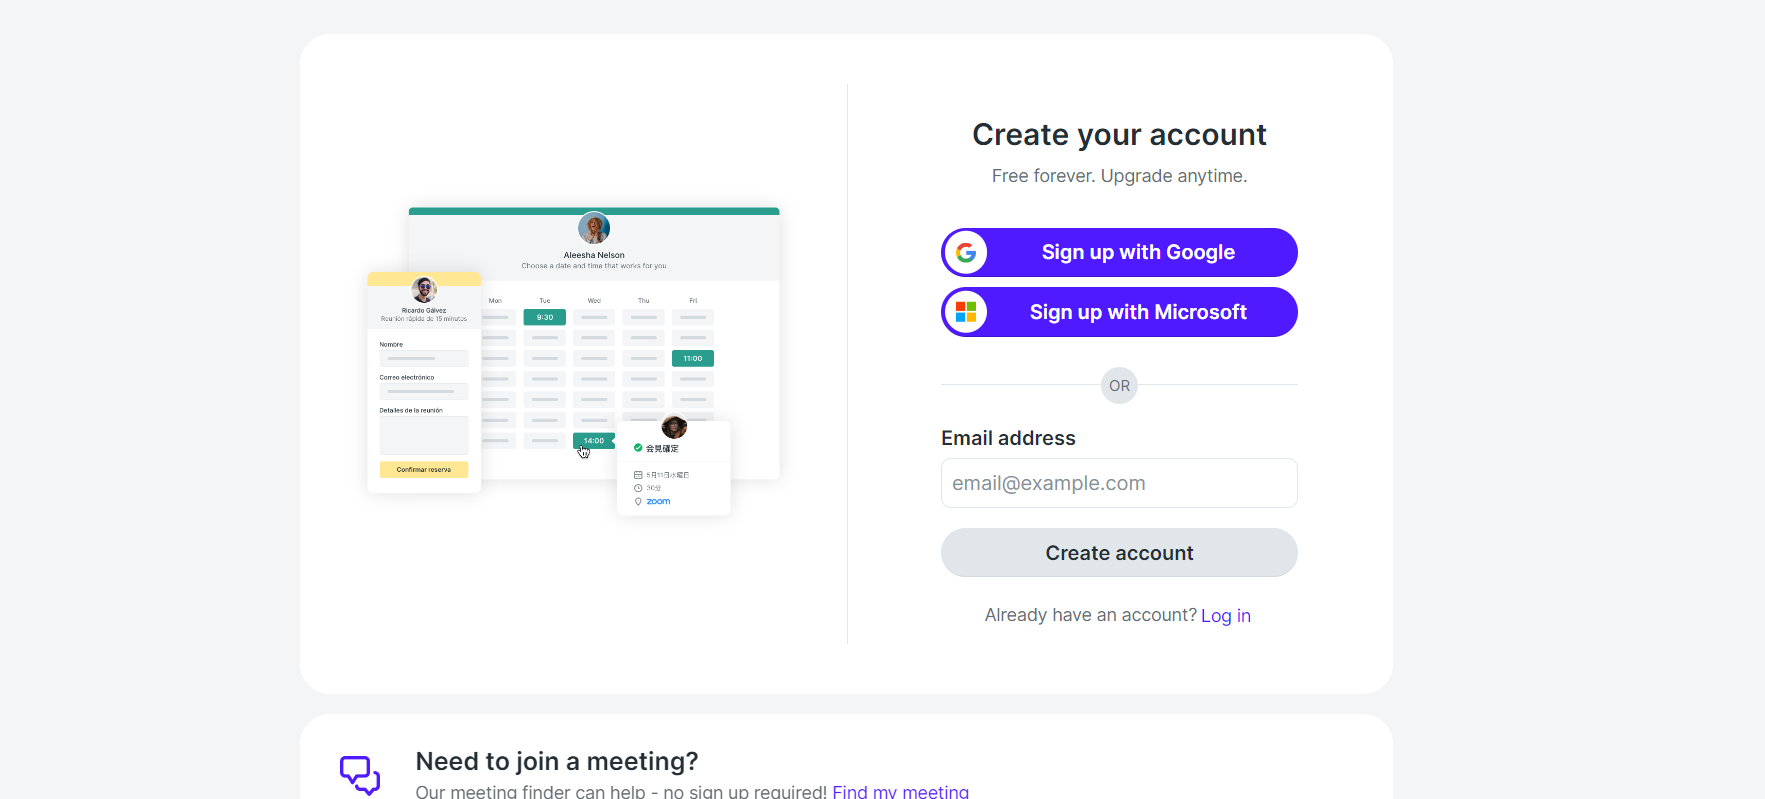
\includegraphics[scale=0.4]{slike/YouCanBookMe-Registracija1.PNG} %veličina slike u odnosu na originalnu datoteku i pozicija slike
	\centering
	\caption{Primjer registracije, klikom na dugme "Create account" kreiramo korisnički račun}
	\label{fig:promjene}
\end{figure}

Korisnik koji se prijavio ima pravo postavljati termine u kojima je slobodan ili se prijavljivati na termine nekih drugih korisnika (zavisi o razlogu zašto koristi "YouCanBookMe" aplikaciju).	U slučaju postavljanja termina odabire koliko mu traje pojedini sastanak sa klijentom te za pojedini dan određuje u kojem vremenu je slobodan il zauzet za sastanak. Ovako slično će u našem primjeru moći raditi zdravstveni djelatnik.

\begin{figure}[H]
	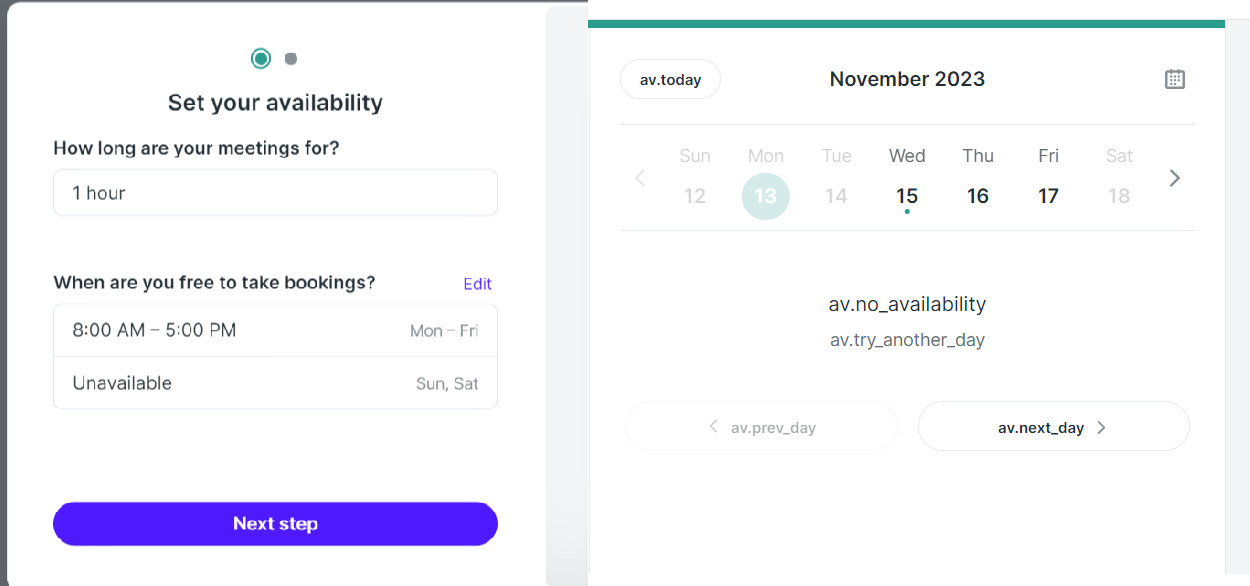
\includegraphics[scale=0.6]{slike/YouCanBookMe-Termin1.PNG} %veličina slike u odnosu na originalnu datoteku i pozicija slike
	\centering
	\caption{Primjer postavljanja dostupnih termina}
	\label{fig:promjene}
\end{figure}

U slučaju da se radi o klijentu koji odabire termin, on ima opciju izabrati samo neke od dostupnih termina. Nakon odabira ispunjava svoje podatke još jedanput kako bi organizator sastanka znao osnovne podatke o klijentu. U našem primjeru će na ovaj način funkcionirati pacijent uz iznimku da neće ponovno morati ispunjavati svoje podatke već će prilikom prijave za dostupni termin njegove osobne podatke moći vidjeti zdravstveni djelatnik. 

\begin{figure}[H]
	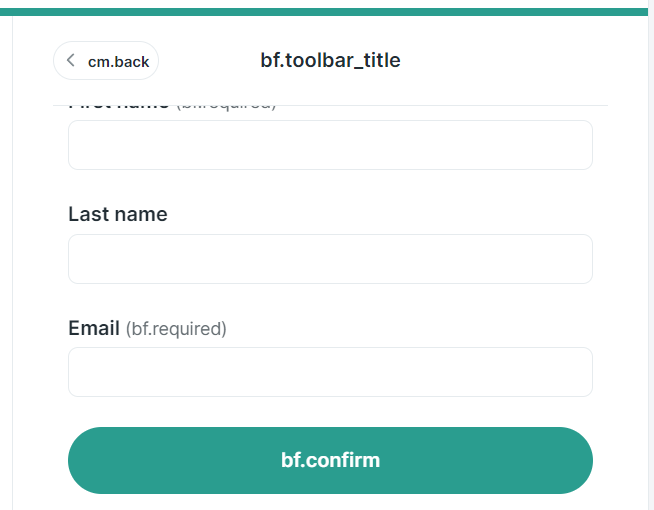
\includegraphics[scale=0.6]{slike/YouCanBookMe-Termin3.PNG} %veličina slike u odnosu na originalnu datoteku i pozicija slike
	\centering
	\caption{Primjer ispunjavanja podataka nakon odabira jednog od dostupnih termina}
	\label{fig:promjene}
\end{figure}

\textbf{\textit{Dodatno pojašnjenje}}\\

Korisnici sustava su:

\begin{packed_item}
	\item \textit{pacijenti}
	\item \textit{zdravstveni djelatnici}
	\item \textit{administrator}
\end{packed_item}

Svaki od te tri skupine korisnika ima različita dopuštenja. Djelatnici ustanove mogu vidjeti sve bolesnike i tretmane koji su im dodijeljeni. Nakon svakog obavljenog postupka djelatnik u sustav registrira pacijenta, a nakon završenog ciklusa zapisuje postignute rezultate. Pacijenti mogu vidjeti samo svoje tretmane. Administrator upravlja čitavim sustavom. Njemu su dostupni svi podaci i može definirati sve što je potrebno za ispravan rad sustava.

Za unesene podatke prilikom registracije u aplikaciju osigurat ćemo provjeru konzistentnosti s podacima iz baze podataka. Nakon toga korisnik postaje pacijent, izabire datum te ima mogućnost otkazati termin 1 dan prije početka tog termina.

Opreme, odnosno uređaji koje posjeduje ustanova se kategoriziraju. Spomenuli smo da slobodni termini ovise o ukupnom kapacitetu opreme/uređaja. Naravno da nije isto ako je čovjeku oštećena ruka ili noga. Tu se radi o drugoj opremi koju će zdravstveni djelatnik morati upotrijebiti za liječenja pacijenta. Dakle, korisnik kojemu je ozljeđena ruka neće zauzimati opremu korisniku kojemu je ozljeđena noga. Očekujemo da će broj oprema/uređaja za određeni dio tijela ipak biti veći od jedan, no svakako će biti ograničen.

Korisnik se u sustav prijavljuje upisivanjem korisničkog imena te svoje lozinke koja mora zadovoljavati određena pravila. Lozinka mora imati minimalno 8 znakova, od čega mora biti minimalno jedno veliko slovo te jedna znamenka. Ako korisnik prilikom registracije i smišljanja lozinke nije zadovoljio navedena pravila, dobit će upozorenje što mu nedostaje za ispravnu lozinku.

Aplikacija će imati 7 stranica koje ćemo sada nabrojati. Na početku sve korisnike (i registrirane i neregistrirane) će dočekati početna naslovna stranica koja će omogućiti korisnicima odlazak na stranicu za registraciju ili prijavu. Neregistrirani korisnici prvo moraju otići na stranicu za registraciju kako bi se mogli prijaviti putem stranice za prijavu. Također ubaciti ćemo stranicu za promjenu lozinke u slučaju da je korisnik zaboravio svoju lozinku. Imati ćemo posebno stranicu za pacijente nakon prijave, stranicu za zdravstvene djelatnike nakon prijave i stranicu za administratore nakon prijave. Pacijenti će na svojoj stranici imati svoje funkcionalnosti poput zakazivanja termina, zdravstveni djelatnici svoje poput potvrde termina, a administratori svoje poput pregleda statistike ili osobnih podataka ostalih korisnika. \\

\textbf{\textit{Opseg projekta}}\\

Na projektu radi 7 osoba, studenata FER-a. Projekt se radi u edukativne svrhe provjere znanja studenata u sklopu predmeta "Programsko inženjerstvo". Vremensko ograničenje za prvu verziju projekta je 7 tjedana, a druga verzija (odnosno cijeli projekt) mora biti isporučen u roku od 14 tjedana od početka rada. Ukupan broj potrošenog vremena otići će najviše na sami rad oko projekta, ali značajan dio vremena otići će i na sastanke uživo gdje će tim redovito raspraviti o tjednom napretku.

\eject
	\chapter{Specifikacija programske potpore}

\section{Funkcionalni zahtjevi}

\noindent \textbf{Dionici:}

\begin{packed_enum}
	
	\item Vlasnik (naručitelj)
	\item Pacijenti
	\item Zdravstveni djelatnici			
	\item Administrator
	\item Razvojni tim
	
\end{packed_enum}


\noindent \textbf{Aktori i njihovi funkcionalni zahtjevi:}


\begin{packed_enum}
	\item  \underbar{Neregistrirani/neprijavljeni korisnik (inicijator) može:}
	
	\begin{packed_enum}
		
		\item se registrirati u sustav kao pacijent te tako stvoriti novi korisnički račun za koji su mu potrebni ime, prezime, korisničko ime, e-mail adresa, OIB, lozinka, spol i datum rođenja.
		\item pregledati naslovnu stranicu koja ga može uputiti na stranicu za registraciju ili stranicu za prijavu
		
		
	\end{packed_enum}
	
	\item  \underbar{Pacijent (inicijator) može:}
	
	\begin{packed_enum}
		
		\item prijaviti se u sustav
		\item odabrati željeni termin dolazaka i opisati svoje zdravstvene poteškoće
		\item otkazati zakazani termin u roku od 24 sata prije samoga termina te potvrditi ili odbiti pomaknuti termin zbog novonastale okolnosti
		\item primati elektroničku poštu o zakazanom terminu i novonastalim okolnostima
		\item pogledati popis svojih prihvaćenih termina te podatke vezane uz termin (doktor koji će ga liječiti, oprema koja će se koristiti, soba u kojoj će se termin odvijati i vrijeme termina)
		
	\end{packed_enum}
	
	
	\item  \underbar{Zdravstveni djelatnik (inicijator) može:}
	
	\begin{packed_enum}
		
		\item prijaviti se u sustav
		\item pregledavati nepotvrđene termine pacijenata u svojoj smjeni
		\item pregledavati potvrđene termine koje on mora odraditi
		\item direktno kontaktirati pacijenta putem elektroničke pošte u slučaju neočekivanih promjena (i predložiti im novi termin)
		\item vidjeti sve pacijente (uključujući njihove osobne podatke) i sve tretmane koji su im dodijeljeni
		\item otkazati zakazani termin u roku od 24 sata prije samoga termina te potvrditi ili odbiti pomaknuti termin zbog novonastale okolnosti
		\item obrisati termin ako smatra da termin nije potrebno izvršit (čime taj termin postaje nevidljiv i ostalim zdravstvenim djelatnicima)
		\item dodijeliti prilikom prihvaćanja termina opremu prikladnu opisu zdravstvenih poteškoća samoga pacijenta (oprema je vezana uz sobu)
		
		
	\end{packed_enum}
	
	
	\item  \underbar{Administrator (inicijator) može:}
	
	\begin{packed_enum}
		
		\item verificirati podatke iz središnjeg informacijskog sustava zdravstvene zaštite
		\item pristupiti popisu korisnika te njihovim osobnim podacima
		\item stvoriti zdravstvenog djelatnika u sustavu
		\item maknuti korisnika iz sustava (i pacijenta i zdravstvenog djelatnika)
		\item pregledavati korisnike (pacijente i zdravstvene djelatnike) i filtrirati ih po nekim parametrima (npr. po spolu)
		
	\end{packed_enum}
	
	\item  \underbar{Baza podataka (sudionik) može:}
	
	\begin{packed_enum}
		
		\item pohraniti podatke o korisnicima i njihovim dopuštenjima
		\item pohraniti podatke o terminima (slobodnim i zauzetim)
		\item pohraniti podatke o opremama/uslugama (slobodnim i zauzetim)
		\item pohraniti podatke o sobama (slobodnim i zauzetim)
		
	\end{packed_enum}
\end{packed_enum}

\eject 



\subsection{Obrasci uporabe}


\noindent \underbar{\textbf{UC1 - Registracija}}
\begin{packed_item}
	
	\item \textbf{Glavni sudionik: }Korisnik
	\item  \textbf{Cilj:} Stvoriti korisnički račun za pacijenta
	\item  \textbf{Sudionici:} Baza podataka
	\item  \textbf{Preduvjet:} -
	\item  \textbf{Opis osnovnog tijeka:}
	
	\item[] \begin{packed_enum}
		
		\item Korisnik odabire opciju za registriranje
		\item Korisnik unosi potrebne podatke
		\item Korisnik pritišće dugme da potvrdi registraciju
		\item Korisnik bude poslan na stranicu za prijavu u sustav
	\end{packed_enum}
	
	\item  \textbf{Opis mogućih odstupanja:}
	
	\item[] \begin{packed_item}
		
		\item[2.a] Odabir zauzetog e-maila i/ili korisničkog imena i/ili OIBa, unos neispravnog e-maila ili unos korisničkog podatka u zabranjenom formatu
		\item[] \begin{packed_enum}
			
			\item Korisnik dobiva obavijest o neuspješnoj registraciji i vraća ga na stranicu za registraciju
			\item Korisnik mijenja krivo unešene podatke ili odustaje od registracije
			
		\end{packed_enum}
		
	\end{packed_item}
\end{packed_item}

\noindent \underbar{\textbf{UC2 - Prijava u sustav}}
\begin{packed_item}
	
	\item \textbf{Glavni sudionici: }Pacijent, Zdravstveni djelatnik, Administrator
	\item  \textbf{Cilj:} Pristupiti uslugama koje pruža naš sustav
	\item  \textbf{Sudionici:} Baza podataka
	\item  \textbf{Preduvjet:} Registracija u sustav
	\item  \textbf{Opis osnovnog tijeka:}
	
	\item[] \begin{packed_enum}
		
		\item Korisnik odabire opciju za prijavu
		\item Korisnik unosi korisničko ime i lozinku
		\item Korisnik pritišće dugme da potvrdi prijavu
		\item Korisnik pristupa uslugama za koje ima dopuštenje (što uključuje odlazak na određenu stranicu - ili za pacijente ili za zdravstvene djelatnike ili za administratore)
	\end{packed_enum}
	
	\item  \textbf{Opis mogućih odstupanja:}
	
	\item[] \begin{packed_item}
		
		\item[2.a] Neispravno korisničko ime i/ili lozinka
		\item[] \begin{packed_enum}
			
			\item Korisnik dobiva obavijest o neuspješnoj prijavi i vraća ga na stranicu za prijavu
			\item Korisnik mijenja krivo unešene podatke ili odustaje od prijave (vraća se na naslovnu stranu)
			
		\end{packed_enum}
		
	\end{packed_item}
\end{packed_item}

\noindent \underbar{\textbf{UC3 - Promjena korisničkih podataka}}
\begin{packed_item}
	
	\item \textbf{Glavni sudionici: }Pacijent, Zdravstveni djelatnik, Administrator
	\item  \textbf{Cilj:} Promijeniti određene korisničke podatke
	\item  \textbf{Sudionici:} Baza podataka
	\item  \textbf{Preduvjet:} Registracija u sustav
	\item  \textbf{Opis osnovnog tijeka:}
	
	\item[] \begin{packed_enum}
		
		\item Korisnik odabire opciju za promjenu podataka
		\item Korisnik unosi podatak ili podatke koje želi promijeniti (email ili korisničko ime ili lozinku)
		\item Korisnik pritišće dugme da potvrdi promjenu podataka
		\item Korisnik pristupa uslugama za koje ima dopuštenje ali s novim podatcima pri čemu stari podatci budu obrisani
	\end{packed_enum}
	
	\item  \textbf{Opis mogućih odstupanja:}
	
	\item[] \begin{packed_item}
		
		\item[2.a] Neispravan oblik email-a ili neispravan oblik lozinke
		\item[] \begin{packed_enum}
			
			\item Korisnik dobiva obavijest o neuspješnoj promijeni podataka te bude vraćen na stranicu za promjenu podataka
			\item Korisnik mijenja krivo unešene podatke ili odustaje od promjene podataka (vraća se na određenu stranicu)
			
		\end{packed_enum}
		
	\end{packed_item}
\end{packed_item}


\noindent \underbar{\textbf{UC4 - Upravljanje terminima}}\\
Uključuje obrasce uporabe UC4.1 Zakazivanje termina, UC4.2 Otkazivanje termina i UC4.3 Pregled termina.\\

\noindent \underbar{\textbf{UC4.1 - Zakazivanje termina}}
\begin{packed_item}
	
	\item \textbf{Glavni sudionik: }Pacijent
	\item  \textbf{Cilj:} Mogućnost odabira termina za odlazak na fizikalnu terapiju
	\item  \textbf{Sudionici:} Baza podataka
	\item  \textbf{Preduvjet:} Korisnik prijavljen kao pacijent
	\item  \textbf{Opis osnovnog tijeka:}
	
	\item[] \begin{packed_enum}
		
		\item Pacijent odabire opciju za zakazivanje termina
		\item Pacijent na prikazanom kalendaru izabire poželjni slobodni termin
		\item Pacijent navodi vrstu i opis oboljenja
		\item Pacijent pritišće dugme za potvrdu odabranog termina
		\item Pacijent dobiva potvrdu o uspješno poslanom zahjevu za termin te bude vraćen na stranicu za pacijente
	\end{packed_enum}
	
	\item  \textbf{Opis mogućih odstupanja:}
	
	\item[] \begin{packed_item}
		
		\item[2.a] Pacijent je unio termin koji ima identično vrijeme održavanja kao i neki već prethodno potvrđeni njegov termin
		\item[] \begin{packed_enum}
			
			\item Pacijent dobiva obavijest da unese drugi termin
			
		\end{packed_enum}
		
		
		\item[2.b] Pacijent je unio termin u roku od 10 sekundi od prethodno poslanog termina
		\item[] \begin{packed_enum}
			
			\item Pacijent dobiva obavijest da pričeka 10 sekundi
			
		\end{packed_enum}
		
		\item[3.a] Pacijent nije unio opis oboljenja a kliknuo je na potvrdu termina
		\item[] \begin{packed_enum}
			
			\item Pacijent dobiva obavijest da unese opis oboljenja
			
		\end{packed_enum}
		
		
		
	\end{packed_item}
\end{packed_item}

\noindent \underbar{\textbf{UC4.2 - Otkazivanje termina}}
\begin{packed_item}
	
	\item \textbf{Glavni sudionik: }Pacijent
	\item  \textbf{Cilj:} Mogućnost otkazivanja termina 
	\item  \textbf{Sudionici:} Baza podataka
	\item  \textbf{Preduvjet:} Korisnik prijavljen kao pacijent i ima zakazan određen termin
	\item  \textbf{Opis osnovnog tijeka:}
	
	\item[] \begin{packed_enum}
		
		\item Pacijent na popisu svojih termina odabire zakazani termin koji želi otkazati
		\item Pacijent odabire opciju za otkazivanje odabranog termina
		\item Pacijent dobije obavijest o uspješno otkazanom terminu
	\end{packed_enum}
	
	\item  \textbf{Opis mogućih odstupanja:}
	
	\item[] \begin{packed_item}
		
		\item[2.a] Pacijent prekasno pokušava otkazati termin (unutar 24 sata kada je zakazani termin)
		\item[] \begin{packed_enum}
			
			\item Sustav onemogućuje pacijentu otkazivanje tog termina te pacijent dobiva obavijest o nemogućnosti otkazivanja termina
			
		\end{packed_enum}
		
	\end{packed_item}
\end{packed_item}

\noindent \underbar{\textbf{UC4.3 - Pregled termina}}
\begin{packed_item}
	
	\item \textbf{Glavni sudionik: }Pacijent
	\item  \textbf{Cilj:} Mogućnost prikaza zakazanih termina
	\item  \textbf{Sudionici:} Baza podataka
	\item  \textbf{Preduvjet:} Korisnik prijavljen kao pacijent
	\item  \textbf{Opis osnovnog tijeka:}
	
	\item[] \begin{packed_enum}
		
		\item Pacijent na kalendaru može vidjeti svoje zakazane termine
	\end{packed_enum}
\end{packed_item}


\noindent \underbar{\textbf{UC5 - E-mail podsjetnik za termin}}
\begin{packed_item}
	
	\item \textbf{Glavni sudionik: }-
	\item  \textbf{Cilj:} Slanje e-mail podsjetnika za zakazani termin (24 sata prije termina)
	\item  \textbf{Sudionici:} Baza podataka, pacijent
	\item  \textbf{Preduvjet:} Korisnik prijavljen kao pacijent i postoji zakazani termin
	\item  \textbf{Opis osnovnog tijeka:}
	
	\item[] \begin{packed_enum}
		
		\item Pacijent dobiva e-mail obavijest o zakazanom terminu (koji je potvrđen od strane određenog zdravstvenog djelatnika)
	\end{packed_enum}
\end{packed_item}

\noindent \underbar{\textbf{UC6: Pregled svih neprihvaćenih termina u djelatnikovoj smjeni}}
\begin{packed_item}
	
	\item \textbf{Glavni sudionik: }Zdravstveni djelatnik
	\item  \textbf{Cilj:} Omogućiti pregled svih neprihvaćenih termina, ali isključivo u djelatnikovoj smjeni
	\item  \textbf{Sudionici:} Baza podataka
	\item  \textbf{Preduvjet:} Korisnik prijavljen kao zdravstveni djelatnik
	\item  \textbf{Opis osnovnog tijeka:}
	
	\item[] \begin{packed_enum}
		
		\item Zdravstvenom djelatniku se na njegovoj stranici pokazuje tablica svih neprihvaćenih termina koje on ima pravo prihvatiti
		\item Zdravstveni djelatnik pritiskom na dostupno dugme šalje taj termin u daljnju konfiguraciju
	\end{packed_enum}
\end{packed_item}

\noindent \underbar{\textbf{UC7 - Pregled svojih rezerviranih termina}}\\
Uključuje obrasce uporabe UC7.1 Odabir opreme, UC7.2 Pomicanje svojih rezerviranih termina, UC7.3 Otkazivanje rezerviranih termina i UC7.4 Brisanje rezerviranih termina\\

\noindent \underbar{\textbf{UC7.1 - Odabir opreme}}
\begin{packed_item}
	
	\item \textbf{Glavni sudionik: }Zdravstveni djelatnik
	\item  \textbf{Cilj:} Omogućiti zdravstvenom djelatniku da odabere opremu koja je prigodna za korištenje s obzirom na opis zdravstvenih problema pacijenta
	\item  \textbf{Sudionici:} Baza podataka
	\item  \textbf{Preduvjet:} Korisnik prijavljen kao zdravstveni djelatnik
	\item  \textbf{Opis osnovnog tijeka:}
	
	\item[] \begin{packed_enum}
		
		\item Zdravstveni djelatnik odabire opremu kojom će liječiti pacijenta
		\item Oprema automatski bude povezana sa sobom 
		\item Zdravstveni djelatnik pritiskom na dugme potvrđuje korištenje opreme u određenoj sobi za tretman
	\end{packed_enum}
	
	\item  \textbf{Opis mogućih odstupanja:}
	
	\item[] \begin{packed_item}
		
		\item[1.a] Svaka instanca te opreme je u to vrijeme zauzeta
		\item[] \begin{packed_enum}
			
			\item Zdravstveni djelatnik će morati ili premjestiti termin ili pokušati liječiti pacijenta nekom drugom opremom
			
		\end{packed_enum}
	
	\end{packed_item}
\end{packed_item}


\noindent \underbar{\textbf{UC7.2 - Pomicanje svojih rezerviranih termina}}
\begin{packed_item}
	
	\item \textbf{Glavni sudionik: }Zdravstveni djelatnik
	\item  \textbf{Cilj:} Omogućiti zdravstvenom djelatniku da pomakne rezervirane termine zbog novonastale okolnosti te čeka potvrdu ili odbijanje od strane pacijenta (to ne smije činiti u istom danu kada je taj termin zakazan, mora biti na vrijeme organiziran)
	\item  \textbf{Sudionici:} Baza podataka
	\item  \textbf{Preduvjet:} Korisnik prijavljen kao zdravstveni djelatnik
	\item  \textbf{Opis osnovnog tijeka:}
	
	\item[] \begin{packed_enum}
		
		\item Zdravstveni djelatnik na kalendaru odabire zakazani termin koje želi pomaknuti
		\item Zdravstveni djelatnik bira novo vrijeme kada želi održati taj termin
		\item Zdravstveni djelatnik pritiskom na dugme potvrđuje novonastale promjene
	\end{packed_enum}
	
	\item  \textbf{Opis mogućih odstupanja:}
	
	\item[] \begin{packed_item}
		
		\item[2.a] Pacijent odbija novi predloženi termin
		\item[] \begin{packed_enum}
			
			\item Zdravstveni djelatnik ponavlja postupak pomicanja svojih rezerviranih termina (dok se pacijent ne složi sa prijedlogom)
			
		\end{packed_enum}
		\item[2.a] Zdravstveni djelatnik pokušava pomaknuti zakazani termin u vremenu unutar 24 sata kada je zakazani termina
		\item[] \begin{packed_enum}
			
			\item Sustav onemogućuje pomicanje termina i šalje zdravstvenom djelatniku odgovarajuću poruku (zdravstveni djelatnik mora odraditi zakazani termin zbog kasne reakcije)
			
		\end{packed_enum}
		
	\end{packed_item}
\end{packed_item}

\noindent \underbar{\textbf{UC7.3 - Otkazivanje rezerviranih termina}}
\begin{packed_item}
	
	\item \textbf{Glavni sudionik: }Zdravstveni djelatnik
	\item  \textbf{Cilj:} Omogućiti zdravstvenom djelatniku otkazivanje rezerviranih termina
	\item  \textbf{Sudionici:} Baza podataka
	\item  \textbf{Preduvjet:} Korisnik prijavljen kao zdravstveni djelatnik
	\item  \textbf{Opis osnovnog tijeka:}
	
	\item[] \begin{packed_enum}
		
		\item Zdravstveni djelatnik na popisu svojih termina odabire zakazani termin koji želi otkazati
		\item Zdravstveni djelatnik odabire opciju za otkazivanje odabranog termina
		\item Zdravstveni djelatnik dobije obavijest o uspješno otkazanom terminu
	\end{packed_enum}
	
	\item  \textbf{Opis mogućih odstupanja:}
	
	\item[] \begin{packed_item}
		
		\item[2.a] Zdravstveni djelatnik prekasno pokušava otkazati termin (unutar 24 sata kada je zakazani termin)
		\item[] \begin{packed_enum}
			
			\item Sustav onemogućuje zdravstvenom djelatniku otkazivanje tog termina (prisiljen je odraditi taj termin) te dobije obavijest o prekasno pokušaju otkazivanja termina
			
		\end{packed_enum}
		
	\end{packed_item}
	
\end{packed_item}


\noindent \underbar{\textbf{UC7.4 - Brisanje rezerviranih termina}}
\begin{packed_item}
	
	\item \textbf{Glavni sudionik: }Zdravstveni djelatnik
	\item  \textbf{Cilj:} Omogućiti zdravstvenom djelatniku brisanje rezerviranih termina
	\item  \textbf{Sudionici:} Baza podataka
	\item  \textbf{Preduvjet:} Korisnik prijavljen kao zdravstveni djelatnik
	\item  \textbf{Opis osnovnog tijeka:}
	
	\item[] \begin{packed_enum}
		
		\item Zdravstveni djelatnik na popisu svojih termina odabire zakazani termin koji želi obrisati (smatra da taj tretman nema smisla izvršiti niti on niti bilo koji drugi zdravstveni djelatnik)
		\item Zdravstveni djelatnik odabire opciju za brisanje odabranog termina
		\item Zdravstveni djelatnik dobije obavijest o uspješno obrisanom terminu
	\end{packed_enum}
	
		
	\end{packed_item}
	

\noindent \underbar{\textbf{UC8 - Pregled termina pacijenata}}
\begin{packed_item}
	
	\item \textbf{Glavni sudionik: }Zdravstveni djelatnik
	\item  \textbf{Cilj:} Omogućiti zdravstvenom djelatniku da pregleda termina pacijenata
	\item  \textbf{Sudionici:} Baza podataka
	\item  \textbf{Preduvjet:} Korisnik prijavljen kao zdravstveni djelatnik
	\item  \textbf{Opis osnovnog tijeka:}
	
	\item[] \begin{packed_enum}
		
		\item Zdravstveni djelatnik upisuje ime, prezime i OIB pacijenta
		\item Zdravstveni djelatnik ima uvid u sve termine tog pacijenta (čak i one termine koji nisu pod njegovoj nadležnosti)
	\end{packed_enum}
	
\end{packed_item}

\noindent \underbar{\textbf{UC9 - Proizvoljno slanje emaila}}
\begin{packed_item}
	
	\item \textbf{Glavni sudionik: }Zdravstveni djelatnik
	\item  \textbf{Cilj:} Omogućiti zdravstvenom djelatniku da komunicira s pacijentom preko elektroničke pošte
	\item  \textbf{Sudionici:} Baza podataka
	\item  \textbf{Preduvjet:} Korisnik prijavljen kao zdravstveni djelatnik
	\item  \textbf{Opis osnovnog tijeka:}
	
	\item[] \begin{packed_enum}
		
		\item Zdravstveni djelatnik odabire opciju slanja emaila
		\item Zdravstveni djelatnik upisuje email adresu određenog pacijenta
		\item Zdravstveni djelatnik upisuje naslov i glavni dio teksta
	\end{packed_enum}
	
\end{packed_item}

\noindent \underbar{\textbf{UC10 - Upravljanje korisnicima}}\\
\textit{Uključuje obrasce uporabe UC10.1. Pregled korisnika, UC10.2. Dodavanje korisnika, UC10.3. Brisanje korisnika.}\\

\noindent \underbar{\textbf{UC10.1. - Pregled korisnika}}
\begin{packed_item}
	
	\item \textbf{Glavni sudionik: }Administrator
	\item  \textbf{Cilj:} Pregledati registrirane korisnike (pacijente i zdravstvene djelatnike)
	\item  \textbf{Sudionici:} Baza podataka
	\item  \textbf{Preduvjet:} Korisnik je registriran i ima prava administratora
	\item  \textbf{Opis osnovnog tijeka:}
	
	\item[] \begin{packed_enum}
		
		\item Korisnik koji je dobio ulogu administratora odabire opciju pregledavanja korisnika
		\item Administratoru se prikazuje lista svih registriranih korisnika sa njihovim osobnim podatcima (posebno odvojeni pacijenti od zdravstvenih djelatnika)
	\end{packed_enum}
	
\end{packed_item}

\noindent \underbar{\textbf{UC10.2. - Dodavanje zdravstvenih djelatnika}}
\begin{packed_item}
	
	\item \textbf{Glavni sudionik: }Administrator
	\item  \textbf{Cilj:} Omogućiti administratoru stvaranje posebno privilegiranog aktora naše aplikacije - zdravstvenog djelatnika
	\item  \textbf{Sudionici:} Baza podataka
	\item  \textbf{Preduvjet:} Korisnik je registriran i ima prava administratora
	\item  \textbf{Opis osnovnog tijeka:}
	
	\item[] \begin{packed_enum}
		
		\item Korisnik koji je dobio ulogu administratora odabire opciju za dodavanje zdravstvenog djelatnika
		\item Administrator u određenim poljima upisuje podatke o novom zdravstvenom djelatniku
		\item Administrator pritiskom na dugme sprema novounesene promjene
	\end{packed_enum}
	
	\item  \textbf{Opis mogućih odstupanja:}
	
	\item[] \begin{packed_item}
		
		\item[2.a] Administrator upisuje zabranjeni format e-maila, već zauzeti e-mail ili općenito unosi podatke u nedopuštenom formatu
		\item[] \begin{packed_enum}
			
			\item Sustav upozorava administratora o neuspjelom unosu i vraća ga na stranicu za upisivanje novih zdravstvenih djelatnika
			\item Administrator ponovno unosi podatke o zdravstvenom djelatniku (ovaj put u ispravnom formatu) ili odustaje od tog čina
			
		\end{packed_enum}
		
	\end{packed_item}
	
\end{packed_item}


\noindent \underbar{\textbf{UC10.3. - Brisanje korisnika}}
\begin{packed_item}
	
	\item \textbf{Glavni sudionik: }Administrator
	\item  \textbf{Cilj:} Omogućiti administratoru brisanje korisnika (pacijenta ili zdravstvenog djelatnika)
	\item  \textbf{Sudionici:} Baza podataka
	\item  \textbf{Preduvjet:} Korisnik je registriran i ima prava administratora i u bazi podataka imamo barem jednog korisnika
	\item  \textbf{Opis osnovnog tijeka:}
	
	\item[] \begin{packed_enum}
		
		\item Korisnik koji je dobio ulogu administratora odabire opciju pregledavanja korisnika
		\item Administrator za određenog korisnika odabire opciju brisanja tog korisnika
		\item Administrator pritiskom na dugme sprema novounesene promjene
		\item Popis korisnika se administratoru osvježava
	\end{packed_enum}
	
\end{packed_item}

\noindent \underbar{\textbf{UC11 - Verifikacija podataka}}
\begin{packed_item}
	
	\item \textbf{Glavni sudionik: }Administrator
	\item  \textbf{Cilj:} Omogućiti administratoru verificiranje unesenih podataka od strane pacijenata
	\item  \textbf{Sudionici:} Baza podataka
	\item  \textbf{Preduvjet:} Korisnik je registriran i ima prava administratora i u bazi podataka se određeni korisnik prijavio kao pacijent
	\item  \textbf{Opis osnovnog tijeka:}
	
	\item[] \begin{packed_enum}
		
		\item Administrator dobiva obavijest o registraciji novog korisnika
		\item Administrator verificira podatke iz središnjeg informacijskog sustava zdravstvene zaštite
	\end{packed_enum}
	
\end{packed_item}

\noindent \underbar{\textbf{UC12 - Pregled statistike}}
\begin{packed_item}
	
	\item \textbf{Glavni sudionik: }Administrator
	\item  \textbf{Cilj:} Omogućiti administratoru pregledati statistiku (npr. koji je postotak u sustavu pacijenata, a koji zdravstvenih djelatnika)
	\item  \textbf{Sudionici:} Baza podataka
	\item  \textbf{Preduvjet:} Korisnik je registriran i ima prava administratora
	\item  \textbf{Opis osnovnog tijeka:}
	
	\item[] \begin{packed_enum}
		
		\item Administrator odabire opciju "Statistika"
		\item Administrator se prikazuju razni statistički podatci (postotak pacijenata u sustavu, postotak zdravstvenih djelatnika u sustavu, postotak pacijenata kojemu treba određena oprema/usluga...)
	\end{packed_enum}
	
\end{packed_item}



\subsubsection{Dijagrami obrazaca uporabe}

\begin{figure}[H]
	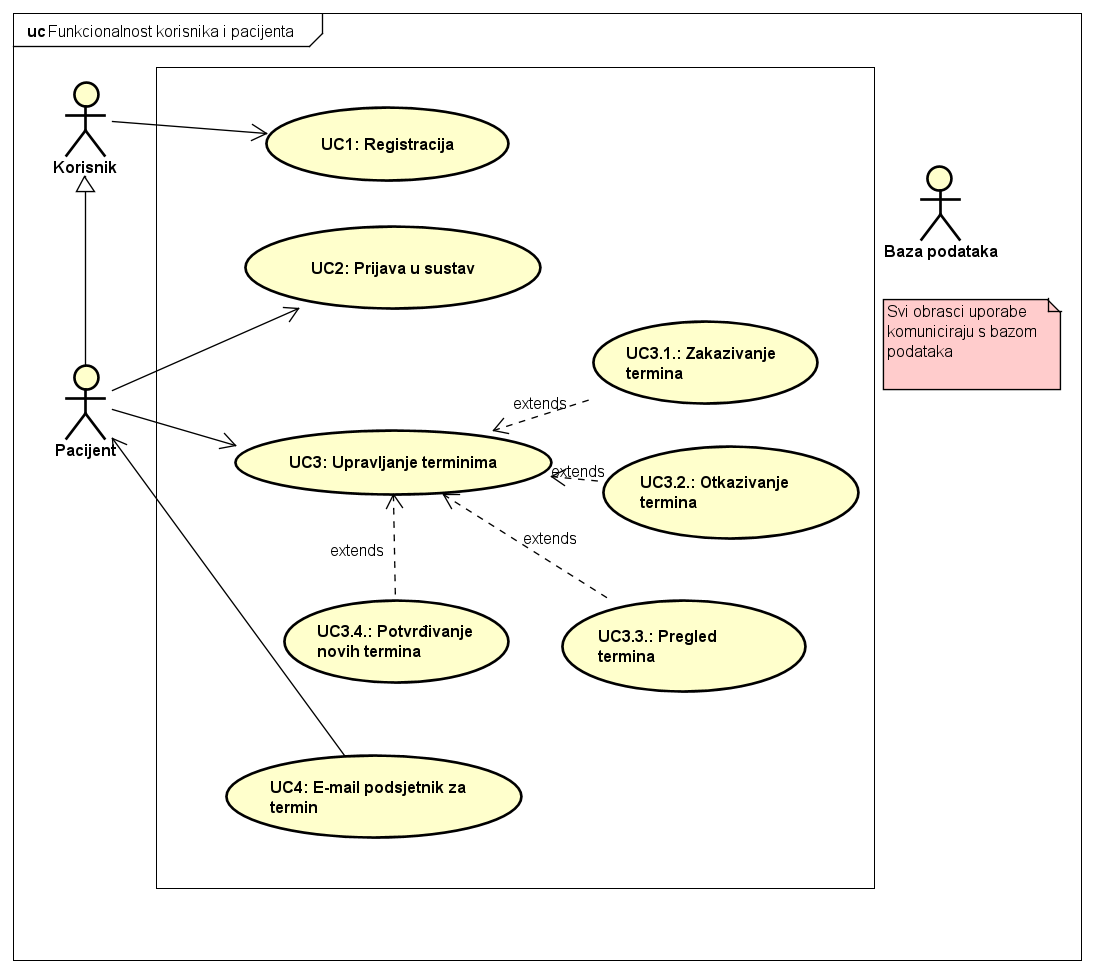
\includegraphics[scale=0.6]{slike/KorisnikIPacijent.PNG} %veličina slike u odnosu na originalnu datoteku i pozicija slike
	\centering
	\caption{Dijagram obrasca uporabe koji prikazuje funkcionalnost korisnika i pacijenta}
	\label{fig:promjene}
\end{figure}

\begin{figure}[H]
	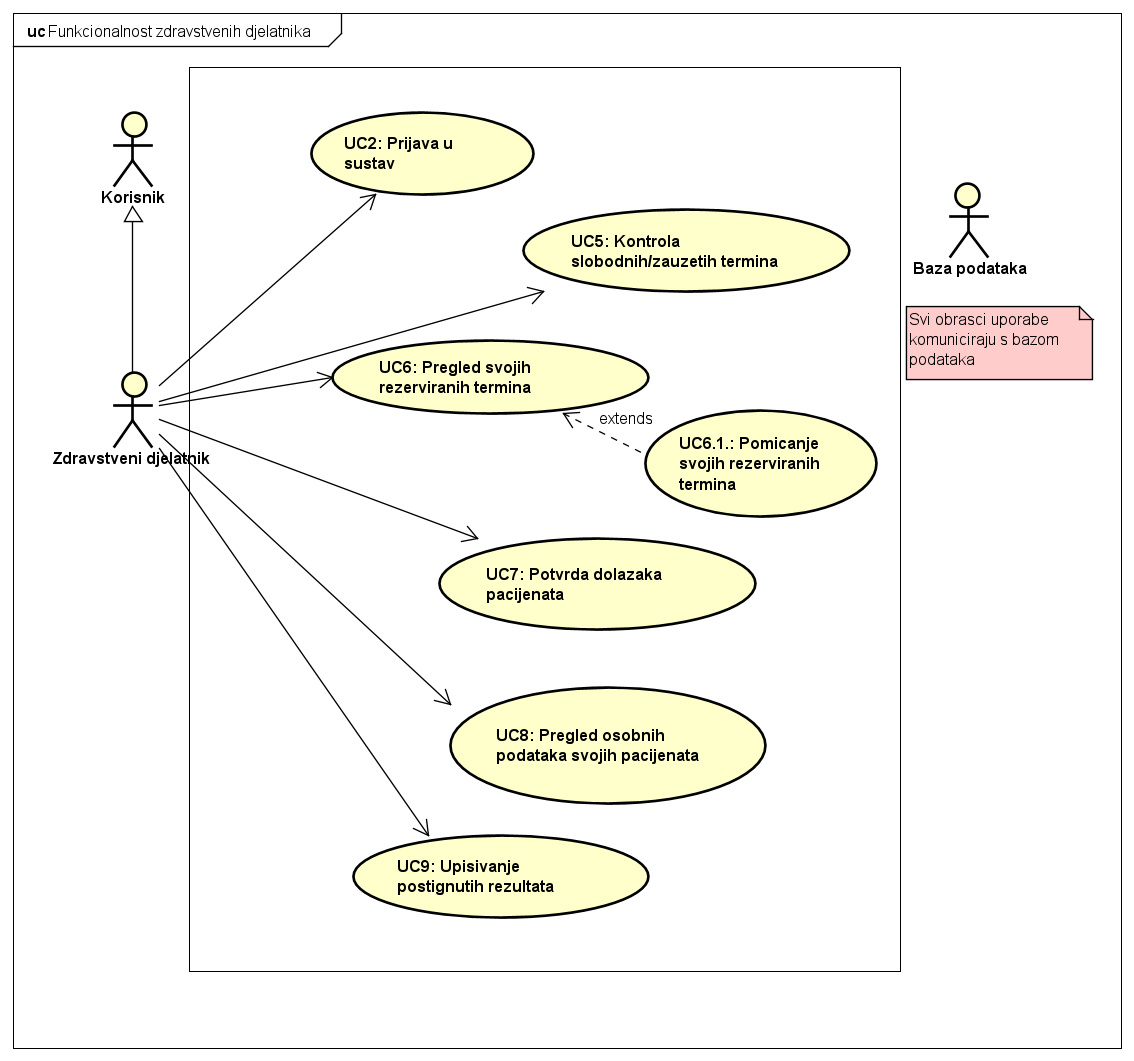
\includegraphics[scale=0.6]{slike/ZdravstveniDjelatnik.PNG} %veličina slike u odnosu na originalnu datoteku i pozicija slike
	\centering
	\caption{Dijagram obrasca uporabe koji prikazuje funkcionalnost zdravstvenih djelatnika}
	\label{fig:promjene}
\end{figure}

\begin{figure}[H]
	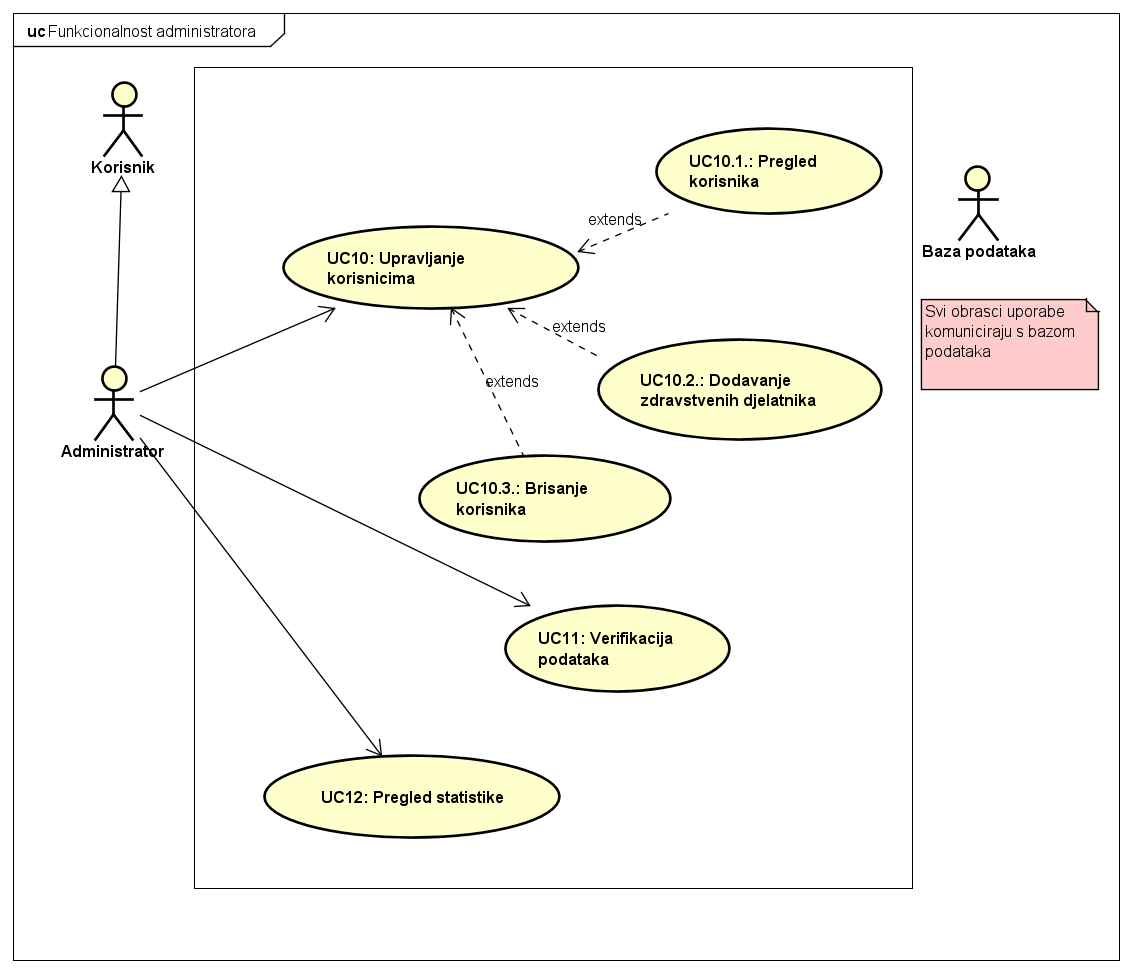
\includegraphics[scale=0.6]{slike/Administrator.PNG} %veličina slike u odnosu na originalnu datoteku i pozicija slike
	\centering
	\caption{Dijagram obrasca uporabe koji prikazuje funkcionalnost administratora}
	\label{fig:promjene}
\end{figure}

\newpage
\subsection{Sekvencijski dijagrami}

\textbf{\text{UC3.1. - Zakazivanje termina}}\\

Korisnik, prijavljen kao pacijent, želi odabrati novi slobodni termin. Poslužitelj dohvaća trenutne termine te korisniku prikazuje kalendar. Pacijent navodi datum i vrijeme kada želi zakazati termin te od strane poslužitelja dobiva pregled svih vlastitih opisa zdravstvenih problema koje je unosio u prošlosti (ako ih ima). Pacijent odabire referencu na ponovljeni opis problema te potvrđuje odabrani termin. Termin se tada sprema u bazu podataka kao nepotvrđeni zahtjev za terminom. Djelatnik dohvaća sve zahtjeve koji odgovaraju njegovoj smjeni te odabire termin koji želi potvrditi. Djelatnik navodi opremu koja mu je potrebna za opisani zdravstveni problem te se vrši provjera dostupnosti opreme. Ako je oprema slobodna, termin se sprema u bazu podataka, djelatnik dobiva potvrdu o spremanju te se pacijentu šalje e-mail o uspješno zakazanom terminu. Ako nema slobodne opreme, djelatnik dobiva listu slobodnih termina u sljedećih tjedan dana te odabire neki od ponuđenih termina, nakon čega se termin sprema u bazu podataka, a djelatnik i pacijent dobivaju prikladnu obavijest.\newline Ako je pacijent unio podatke o novom zdravstvenom problemu, poslužitelj te informacije sprema u bazu podataka. Pacijent potvrđuje odabrani termin te se on sprema kao nepotvrđeni zahtjev za terminom. Postupak je dalje jednak kao i u prijašnjem slučaju - Djelatnik dohvaća sve zahtjeve koji odgovaraju njegovoj smjeni te odabire termin koji želi potvrditi. Djelatnik navodi opremu koja mu je potrebna za opisani zdravstveni problem te se vrši provjera dostupnosti opreme. Ako je oprema slobodna, termin se sprema u bazu podataka, djelatnik dobiva potvrdu o spremanju te se pacijentu šalje e-mail o uspješno zakazanom terminu. Ako nema slobodne opreme, djelatnik dobiva listu slobodnih termina u sljedećih tjedan dana te odabire neki od ponuđenih termina, nakon čega se termin sprema u bazu podataka, a djelatnik i pacijent dobivaju prikladnu obavijest.

\begin{figure}[H]
	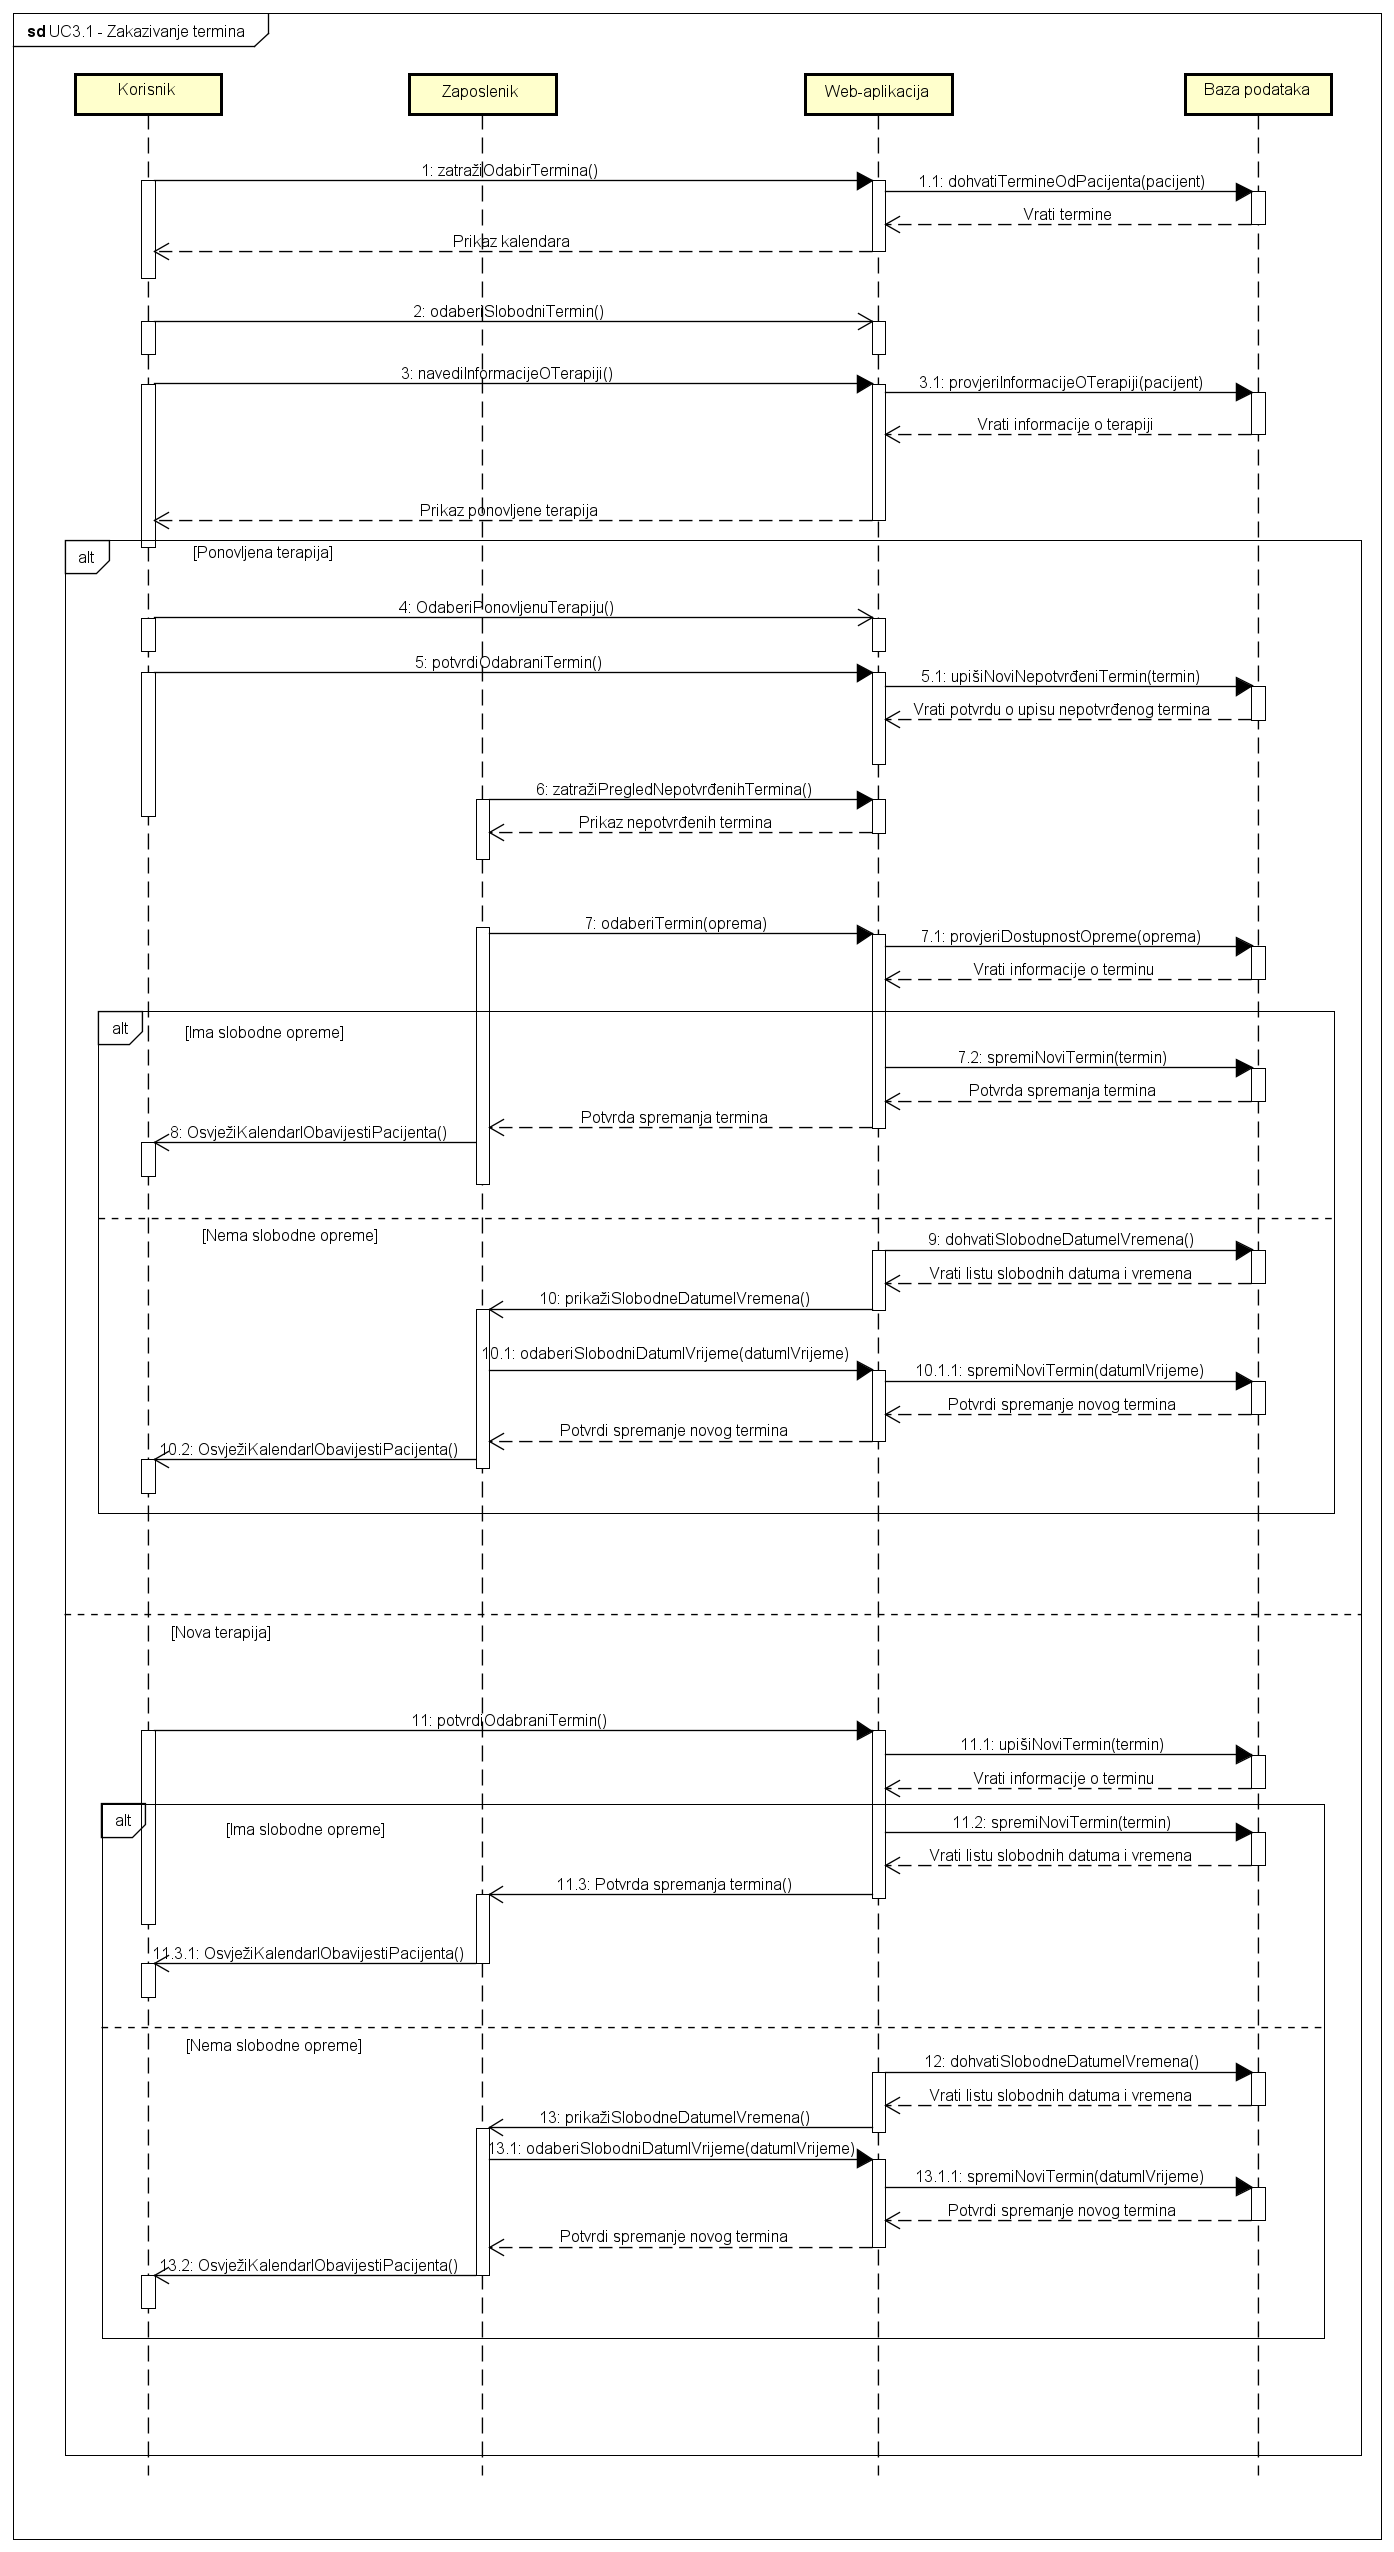
\includegraphics[scale=0.33]{slike/zakazivanjeTerminaUC3.1}
	\centering
	\caption{Sekvencijski dijagram za UC3.1.}
\end{figure}

\newpage

\textbf{\text{UC3.2. - Otkazivanje termina}}\\

Korisnik, prijavljen kao pacijent, želi odabrati termin kako bi ga mogao otkazati. Poslužitelj dohvaća sve zakazane termine od tog pacijenta i prikazuje ih u kalendaru. Pacijent otkazuje odabrani termin. Poslužitelj ispituje ispravnost odabranog termina te ako je on ispravan, briše ga iz baze podataka, osvježava kalendar i šalje e-mail poruku pacijentu. Ako pacijent prekasno pokušava otkazati termin, odnosno ako to čini 24 sata prije zakazanog termina, poslužitelj ne briše termin i šalje odgovarajuću poruku pacijentu.

\begin{figure}[H]
	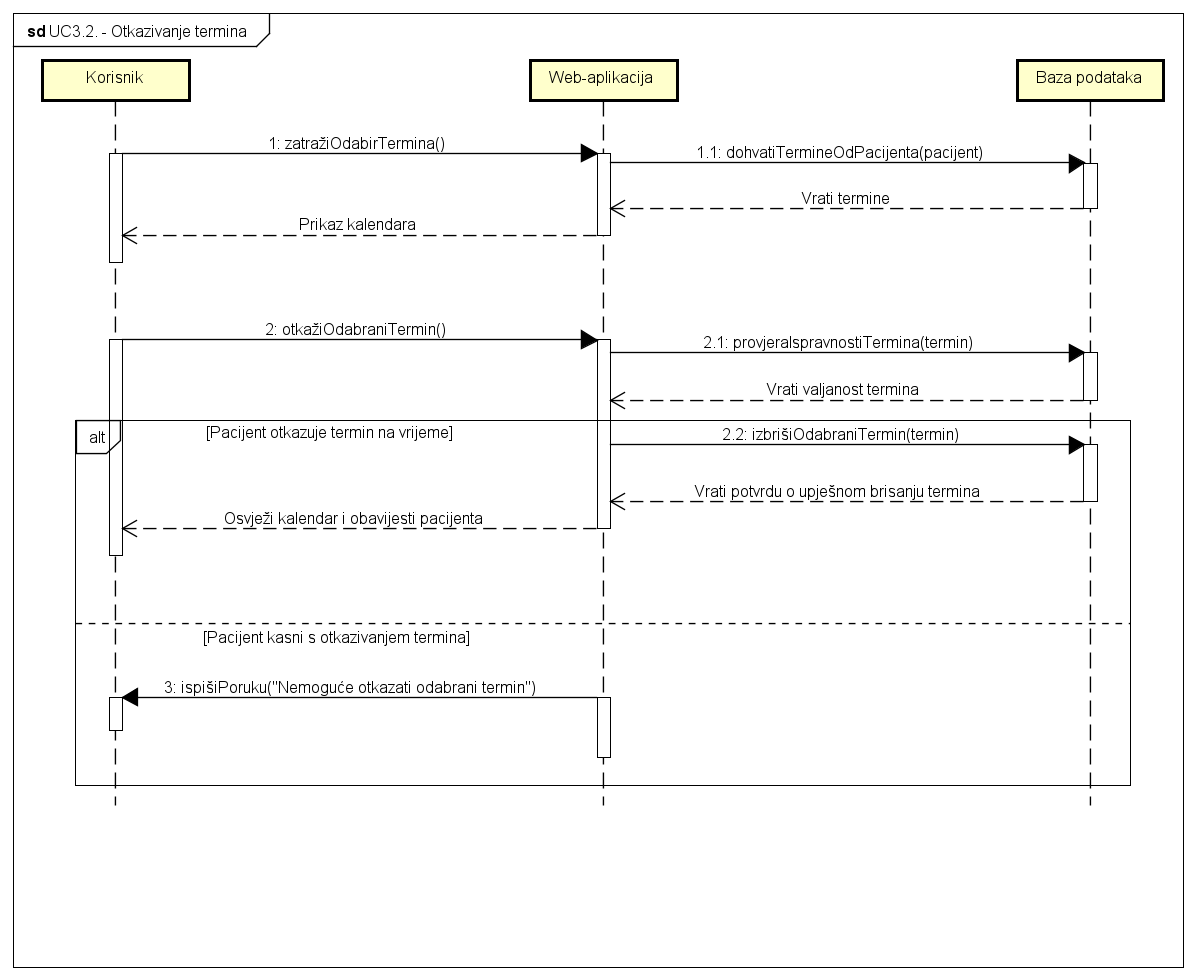
\includegraphics[scale=0.5]{slike/UC3.2_Otkazivanje_termina}
	\centering
	\caption{Sekvencijski dijagram za UC3.2.}
\end{figure}

\newpage

\textbf{\text{UC6.1 - Pomicanje svojih rezerviranih termina}}\\

Korisnik, prijavljen kao zdravstveni djelatnik, želi premjestiti svoje rezervirane termine zbog nemogućnosti njihovog izvršavanja. Poslužitelj dohvaća sve rezervirane termine od zdravstvenog djelatnika te ih prikazuje na kalendaru. Zdravstveni djelatnik odabire sve termine koje bi želio premjestiti. Sljedeći koraci se izvršavaju sve dok se ne obrade svi odabrani termini. Dok se ne dobije potvrda pacijenta, zdravstveni djelatnik odabire opciju otkazivanja trenutno odabranog termina. Poslužitelj ispituje ispravnost odabranog termina te vraća njegovu valjanost. Ako je zdravstveni djelatnik na vrijeme odlučio pomaknuti odabrani termin, on to čini te se pacijentu šalje obavijest o mogućem novom terminu. Ako zdravstveni djelatnik pomiče odabrani termin unutar 24 sata od samoga odabranoga termina, poslužitelj ga u tome onemogućuje. Nakon što pacijent potvrdi suglasnost o novome terminu, zdravstveni djelatnik potvrđuje samu promjenu termina. Poslužitelj dobiva i stari i novi termin te se stari uklanja, a novi dodaje u bazu podataka. Nakon pomicanja termina, zdravstvenom se djelatniku osvježava kalendar.

\begin{figure}[H]
	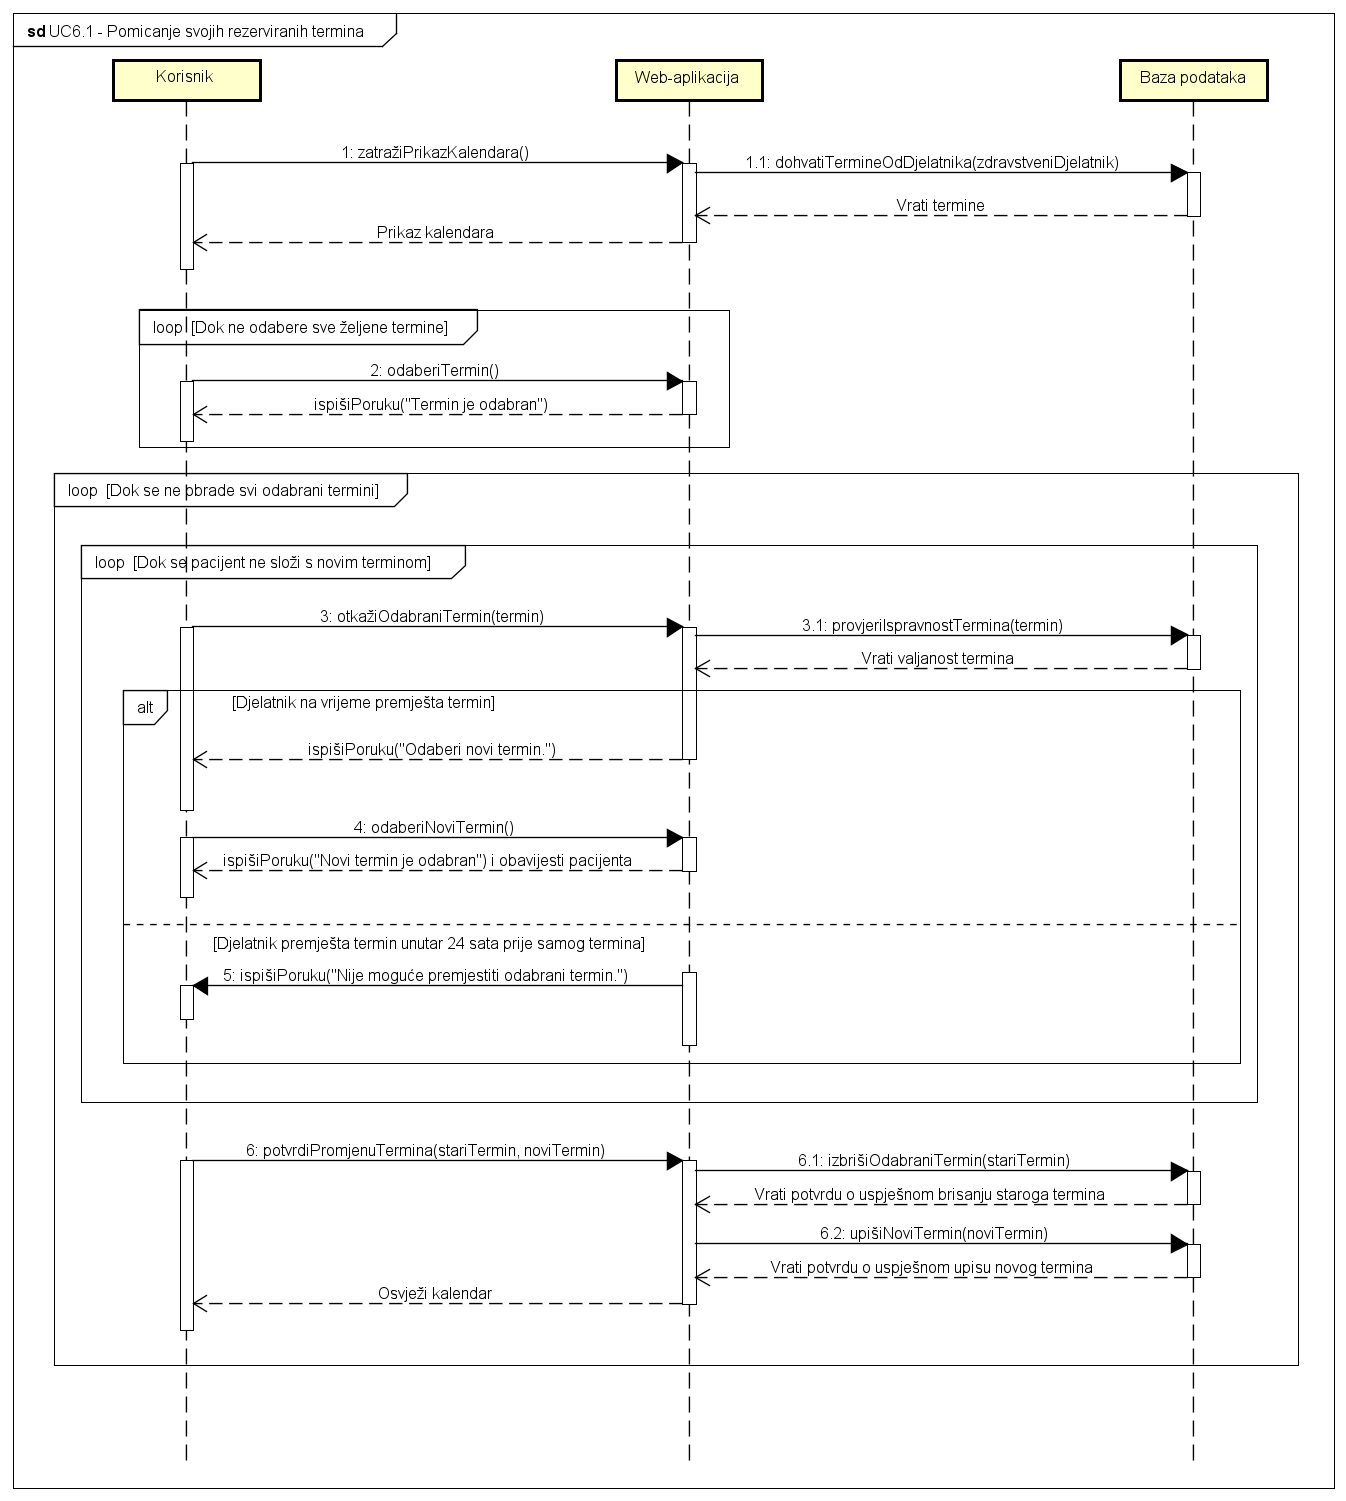
\includegraphics[scale=0.5]{slike/UC6.1_Pomicanje_svojih_rezerviranih_termina}
	\centering
	\caption{Sekvencijski dijagram za UC6.1}
\end{figure}

\section{Ostali zahtjevi}

\begin{packed_item}
	\item Korisničko sučelje mora biti intuitivno i prilagođeno, olakšavajući korisnicima njenu upotrebu
	\item Sustav mora omogućiti istovremeni rad većem broju korisnika
	\item Sustav treba omogućiti brzu i učinkovitu prijavu pacijenata te raspoređivanje termina unutar radnog vremena
	\item Prilikom komunikacije s bazom podataka, svi osobni podaci moraju biti prikladno zaštićeni
	\item Korisnicko sučelje i sustav moraju podržavati hrvatsku abecedu (dijakritičke znakove) pri unosu i prikazu tekstualnog sadrzaja 
	\item Apikacija mora biti oblikovana poštivajući načela objektno-orijentiranog programiranja
	\item Neispravno koristenje korisničkog sučelja ne smije narušiti funkcionalnost i rad sustava
	\item Sustav treba omogućiti obavještavanje pacijenata putem elektroničke pošte o promjenama u rasporedu ili drugim važnim informacijama
	\item Sistemski administrator treba imati potpuni pristup svim podacima i mogućnost definiranja postavki sustava
\end{packed_item}


			 
			 
	
	\chapter{Arhitektura i dizajn sustava}

		Arhitekturu sustava općenito (pa tako i našeg) možemo podijeliti na tri dijela:
	\begin{itemize}
		\item 	\textit{Web poslužitelj}
		\item 	\textit{Web aplikacija}
		\item 	\textit{Baza podataka}		
	\end{itemize}
	
	\textbf{Internetski preglednik (web preglednik, web browser)} je dio arhitekture koji korisniku omogućuje pregled web-stranica pa tako i samoga sadržaja koji se nalazi na njoj. Korisnik putem web preglednika šalje HTTP zahtjev poslužitelju za dohvat željenog sadržaja i čeka HTTP odgovor. HTTP je protokol bez stanja što znači da primatelj ne smije zadržati stanje sesije iz prethodnih zahtjeva. Neki od popularnijih web preglednika su "Google Chrome" ili "Opera".
	
	\textbf{Web poslužitelj} je osnova svake web aplikacije. On šalje klijentu HTTP odgovor na određeni HTTP zahtjev. Korisnik koristi web aplikaciju na način da web aplikacija obrađuje zahtjev te ovisno o potrebi pristupa bazi podataka. Poslužitelj vraća odgovor u obliku HTML dokumenta koji je vidljiv korisniku.
		
    \begin{figure}[H]
    	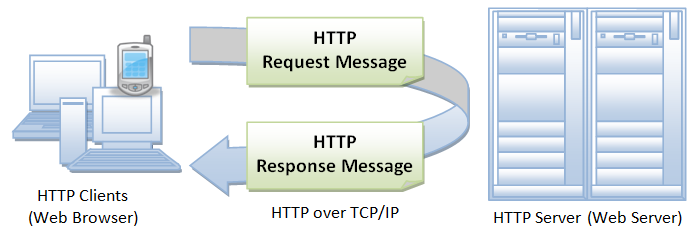
\includegraphics[scale=1.2]{slike/HTTP.PNG} %veličina slike u odnosu na originalnu datoteku i pozicija slike
    	\centering
    	\caption{Prikaz HTTP komunikacije između klijenta i poslužitelja}
    	\label{fig:promjene}
    \end{figure}
    
    \textit{\newline \newline}
    
    Naša grupa je za projekt na predmetu Programsko inženjerstvo (ak.god. 2023./2024.) odabrala React sustav za potrebe frontenda. Odabrali smo React zbog njegove jednostavne i moćne arhitekture koja omogućuje brz i održiv razvoj web aplikacija. React se temelji na principu komponenata, što znači da aplikaciju gradimo kao skup neovisnih dijelova sučelja, svaki s vlastitom logikom i stilovima. Time svaka komponenta postaje ponovno upotrebljiva i lako zamjenjiva što olakšava razvoj aplikacije.
    
    Za backend smo odabrali raditi u programskom jeziku Java i to u Spring Boot-u. Koristili smo Maven alat za izgradnju programskog koda. Spring Boot nam se svidio zbog dvije karakteristike: inverzija kontrole gdje sam Spring Boot kontrolira izvršavanje programskog koda te injektiranje objekata o kojima ovisi rad koda. Neke od karakteristika Spring Boot-a su: unaprijed pripremljene funkcionalnosti, nema generiranja klasa i koda već se koriste unaprijed definirane biblioteke. U svakom slučaju Spring Boot zna dosta olakšati programeru posao. Također olakšava i spajanje na bazu podataka o kojoj će biti više riječi u sljedećoj cjelini.
    
    Razvojno okruženje koje smo koristili zavisilo je od člana do člana ekipe, neki su radili u Eclipse-u, neki u IntelliJ. Koristili smo GitHub sustav za upravljanje verzijama programske potpore te TeXstudio za pisanje dokumentacije.
    
    \begin{figure}[H]
    	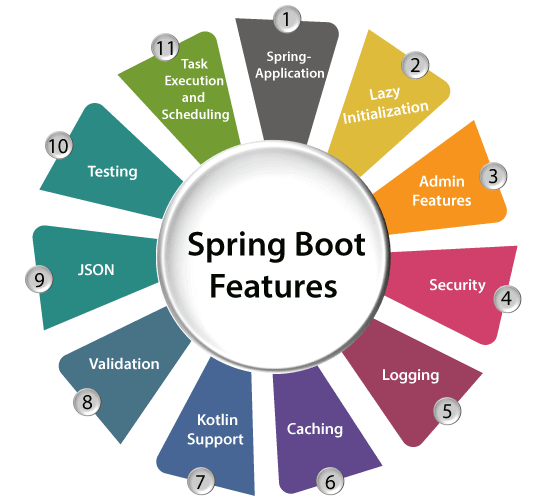
\includegraphics[scale=0.5]{slike/SpringBoot.PNG} %veličina slike u odnosu na originalnu datoteku i pozicija slike
    	\centering
    	\caption{Neke od koristi Spring Boot-a}
    	\label{fig:promjene}
    \end{figure}
		

				
	\section{Baza podataka}
			
		\hspace*{2em}
     	Za bazu podataka odabrali smo SQL vrstu baze podataka, točnije MySql software zbog svoje jednostavnosti i kvalitetne usluge. MySql je besplatni open-source sistem za upravljanje bazama podataka. Također ga podržava velika i aktivna zajednica korisnika što nam omogućava brz pronalazak potrebnih resursa, tutorijala i rješenja za moguće probleme. Što se performanse tiče, MySql je poznat po brzini i efikasnosti te se koristi kako za manje web aplikacije tako i za velike poslovne sisteme. Lako se integrira u različite programske jezike i razvojne okoline.
     	
     	\begin{figure}[H]
     		
\includegraphics[scale=1]{slike/MySql.PNG} %veličina slike u odnosu na originalnu datoteku i pozicija slike
     		\centering
     		\caption{MySql}
     		\label{fig:promjene}
     	\end{figure}
     	
		
		
			\subsection{Opis tablica}
			
				
				\hspace*{2em}
				Glavni cilj: Baza podataka osigurava pregled i pohranu podataka o svim faktorima procesa zauzimanja termina u medicinsko rehabilitacijskoj klinici. Kako bi se osiguralo pravilno rukovanje bazom podataka potrebne su pojedine tablice tj. entiteti od kojih svaki sadrži svoje atribute te odnose među pojedinim entitetima koji se u struci nazivaju „relationships“. Entiteti: Našu bazu podataka tvori nekoliko entiteta, preciznije: User (korisnik), Appointment (dogovoreni sastanak), Equipment (oprema) te Room (prostorija/radna sala). 
				\newline
				\hspace*{2em}
				Entitet User: To je najbitniji entitet jer sadrži podatke o svim djelatnicima medicinsko rehabilitacijske klinike, pacijentima i ostalim djelatnicima. Za ostvarivanje funkcionalnosti potrebni su sljedeći atributi: idUser(primary key), imeUser, prezime, oib, username, password, email, datum rođenja, spol, start date(unosi se pri stvaranju tj. kad je napravljen korisnički račun) te na kraju enum koji specijalizira entitet Usera na jedno od dvije opcije. To su Patient ili Employee. Employee-u se dalje bilježi status, tj. gleda li se na njega kao aktivnog zaposlenika, neaktivnog ili admin.
				\newline
				\hspace*{2em}
				Entitet Appointment: Entitet Appointment prikazuje sve dogovorene sastanke te omogućava uspješno dogovaranje novih bez da dođe do nekih problema kao što su kolizije ili nedostatak opreme. Atributi u entitetu Appointment su: idApp(primary key), vrijeme termina (od kad do kad je zakazan termin), user, opis termina, oprema i prostorija. 
				\newline
				\hspace*{2em}
				Entitet Equipment: Entitet Equipment sadrži podatke o svoj opremi. Osigurava da ne dođe do problema rezerviranja više opreme nego što je dostupno, na primjer pacijent A je rezervirao zadnje štake te pacijent B u istom terminu nema pristup tom komadu opreme. Atributi koji čine entitet Equipment su: idEqu(primary key), ime, opis i status(radi li ili ne). 
				\newline
				\hspace*{2em}
				Entitet Prostorija: Entitet Prostorija prikazuje podatke o mogućim prostorijama za rehabilitaciju. Osigurava da određena prostorija ne može biti zauzeta više puta odjednom. Atributi koji sačinjavaju entitet Prostorija su: idPro(primary key), ime i kapacitet. 
				\newline
				\hspace*{2em}
				Veze (relationships) među entitetima: Veze među entitetima osiguravanju pravilnu i predviđenu funkcionalnost cijelog sustava (web aplikacije), povezuju sve entitete na način koji tvori logiku povezanosti. Uspostavljene su tri veze u našoj bazi podataka: User  Appointment. Veza User - Appointment je one to many(jedan na više, 1 - N) tip veze. Jedan User može zatražiti više sastanaka. Appointment - Prostorija. Veza Appointment  Prostorija je one to many(jedan na više, 1 - N) tip veze. Više sastanaka se može održavati u isto vrijeme u istoj prostoriji. Prostorija - Equipment. Veza Prostorija  Equipment je one to many(jedan na više, 1 - N) tip veze. Više opreme se može držati u jednoj prostoriji.
				
				
				\begin{longtblr}[
					label=none,
					entry=none
					]{
						width = \textwidth,
						colspec={|X[2,l]|X[3.5,l]|X[6,l]|}, 
						rowhead = 1,
					}
					\hline \SetCell[c=3]{c}{\textbf{korisnik - User tablica}} \\ \hline[3pt]
					\SetCell{LightGreen}idUser & INT AUTO\_INCREMENT & Jedinstveni identifikator korisnika \\ \hline
					imeUser & VARCHAR(255) & Ime korisnika \\ \hline
					prezime & VARCHAR(255) & Prezime korisnika \\ \hline
					oib & INT & OIB korisnika \\ \hline
					username & VARCHAR(255) & Korisničko ime \\ \hline
					password & VARCHAR(255) & Lozinka \\ \hline
					datumRodenja & DATE & Datum rođenja \\ \hline
					spol & VARCHAR(1) & Spol (M ili F) \\ \hline
					startDate & DATE & Datum početka korisničkog računa \\ \hline
					email & VARCHAR(255) & E-mail adresa \\ \hline
				\end{longtblr}
				
				
				\begin{longtblr}[
					label=none,
					entry=none
					]{
						width = \textwidth,
						colspec={|X[2.5,l]|X[3.5,l]|X[6,l]|}, 
						rowhead = 1,
					}
					\hline \SetCell[c=3]{c}{\textbf{prostorija - Prostorija tablica}} \\ \hline[3pt]
					\SetCell{LightGreen}idPro & INT AUTO\_INCREMENT & Jedinstveni identifikator prostorije \\ \hline
					imePro & VARCHAR(255) & Ime prostorije \\ \hline
					kapacitet & INT & Kapacitet prostorije \\ \hline
				\end{longtblr}
				
				
				\begin{longtblr}[
					label=none,
					entry=none
					]{
						width = \textwidth,
						colspec={|X[2.5,l]|X[3.5,l]|X[6,l]|}, 
						rowhead = 1,
					}
					\hline \SetCell[c=3]{c}{\textbf{patient - Patient tablica}} \\ \hline[3pt]
					\SetCell{LightGreen}idUser & INT AUTO\_INCREMENT & Jedinstveni identifikator pacijenta \\ \hline
				\end{longtblr}
				
				
				\begin{longtblr}[
					label=none,
					entry=none
					]{
						width = \textwidth,
						colspec={|X[2.5,l]|X[3.5,l]|X[6,l]|}, 
						rowhead = 1,
					}
					\hline \SetCell[c=3]{c}{\textbf{employee - Employee tablica}} \\ \hline[3pt]
					\SetCell{LightGreen}statusEmp & VARCHAR(255) & Status zaposlenika \\ \hline
					idUser & INT AUTO\_INCREMENT & Jedinstveni identifikator zaposlenika \\ \hline
				\end{longtblr}
				
				
				\begin{longtblr}[
					label=none,
					entry=none
					]{
						width = \textwidth,
						colspec={|X[2.5,l]|X[3.5,l]|X[6,l]|}, 
						rowhead = 1,
					}
					\hline \SetCell[c=3]{c}{\textbf{appointment - Appointment tablica}} \\ \hline[3pt]
					\SetCell{LightGreen}idApp & INT AUTO\_INCREMENT & Jedinstveni identifikator termina \\ \hline
					vrijemeTermina & DATETIME & Vrijeme termina \\ \hline
					idUser & INT & Jedinstveni identifikator korisnika \\ \hline
					opisTermina & VARCHAR(255) & Opis termina \\ \hline
					idEqu & INT & Jedinstveni identifikator opreme \\ \hline
					idPro & INT & Jedinstveni identifikator prostorije \\ \hline
				\end{longtblr}
				
				
				\begin{longtblr}[
					label=none,
					entry=none
					]{
						width = \textwidth,
						colspec={|X[2.5,l]|X[3.5,l]|X[6,l]|}, 
						rowhead = 1,
					}
					\hline \SetCell[c=3]{c}{\textbf{equipment - Equipment tablica}} \\ \hline[3pt]
					\SetCell{LightGreen}idEqu & INT AUTO\_INCREMENT & Jedinstveni identifikator opreme \\ \hline
					imeEqu & VARCHAR(255) & Ime opreme \\ \hline
					opisEqu & VARCHAR(255) & Opis opreme \\ \hline
					statusEqu & VARCHAR(255) & Status opreme \\ \hline
					idPro & INT & Jedinstveni identifikator prostorije \\ \hline
				\end{longtblr}
				
			\newpage
			
			\subsection{Dijagram baze podataka}
				 U ovom potpoglavlju potrebno je umetnuti dijagram baze podataka. Primarni i strani ključevi moraju biti označeni, a tablice povezane. Bazu podataka je potrebno normalizirati. Podsjetite se kolegija "Baze podataka".
				
				\begin{figure}[H]
					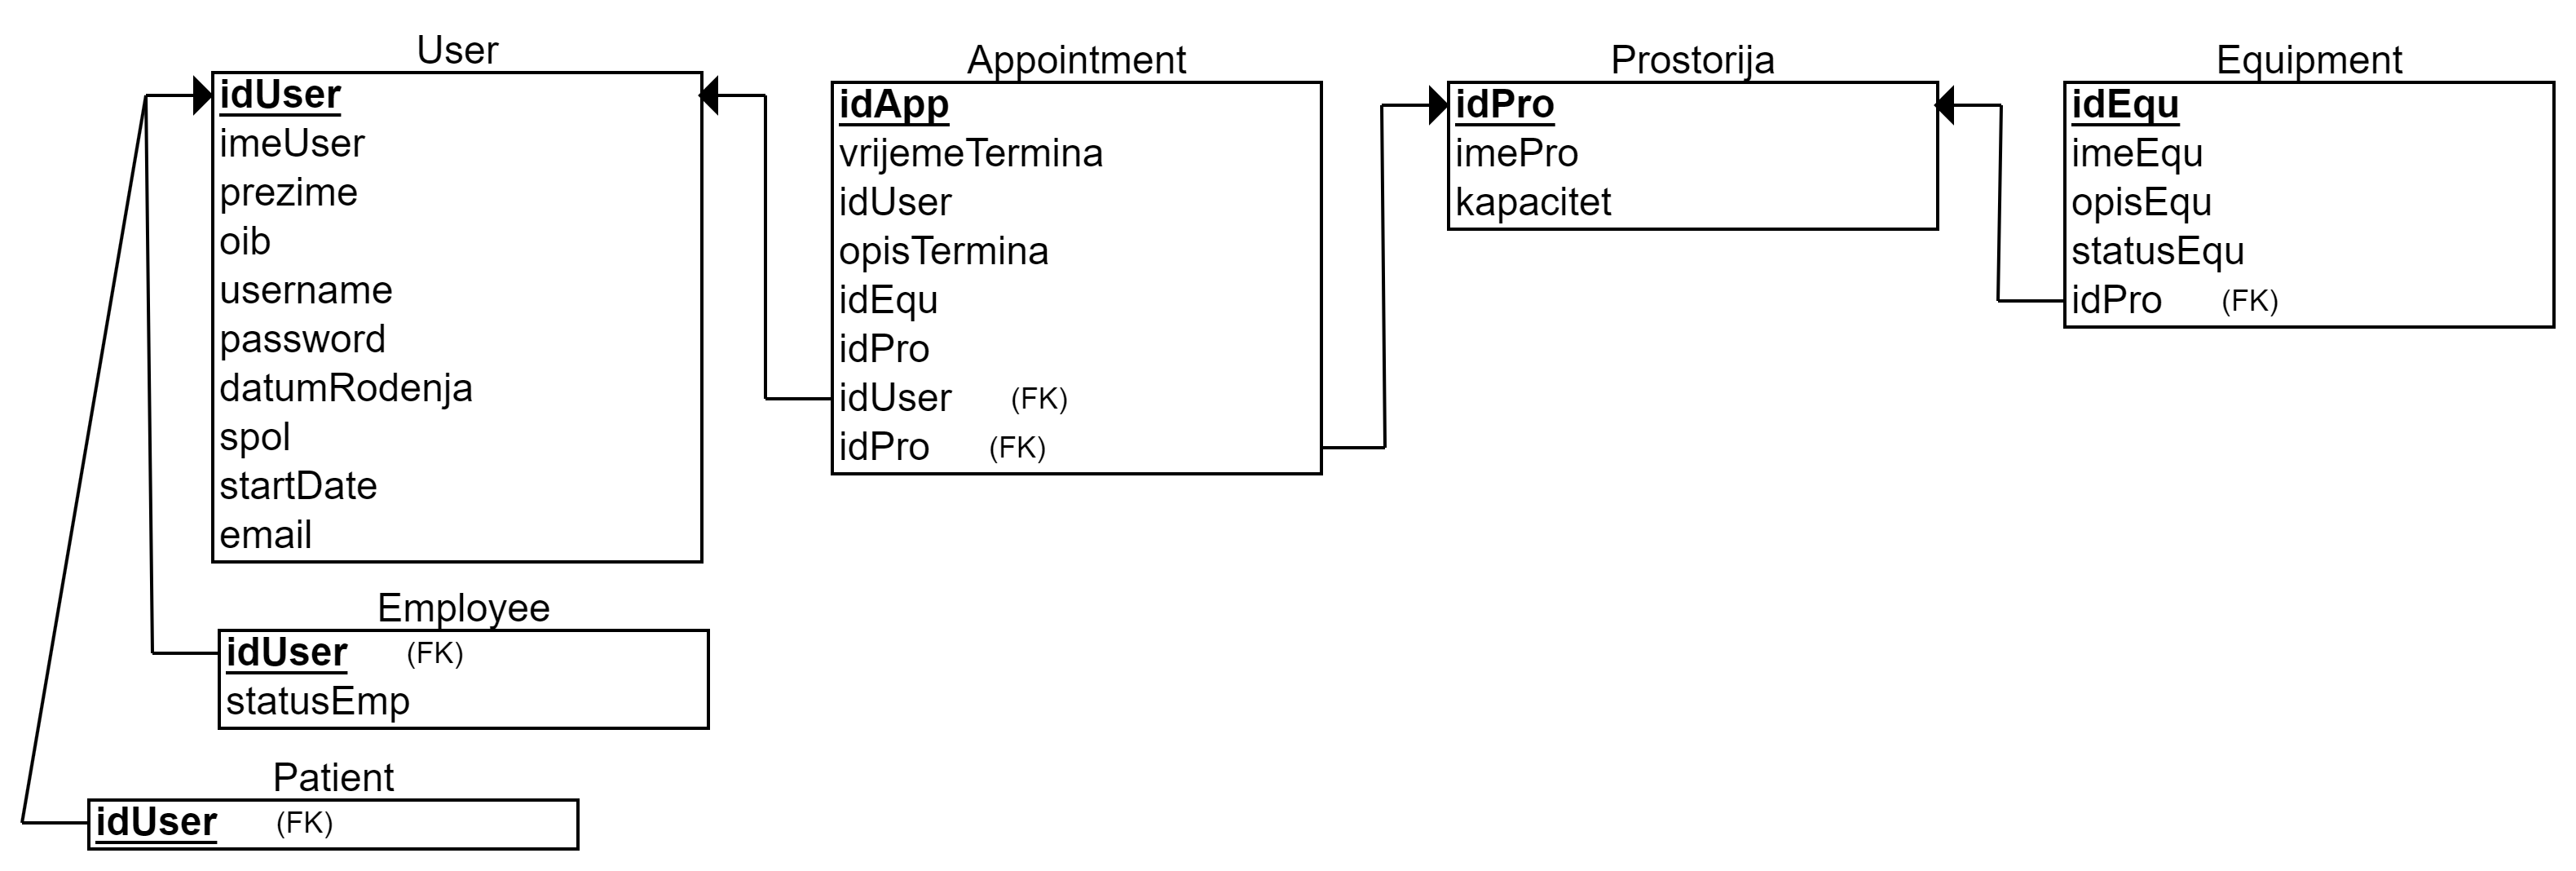
\includegraphics[scale=0.14]{slike/bp_rel.PNG} %veličina slike u odnosu na originalnu datoteku i pozicija slike
					\centering
					\caption{Relacijski model baze podataka}
					\label{fig:promjene}
				\end{figure}
				
				\begin{figure}[H]
					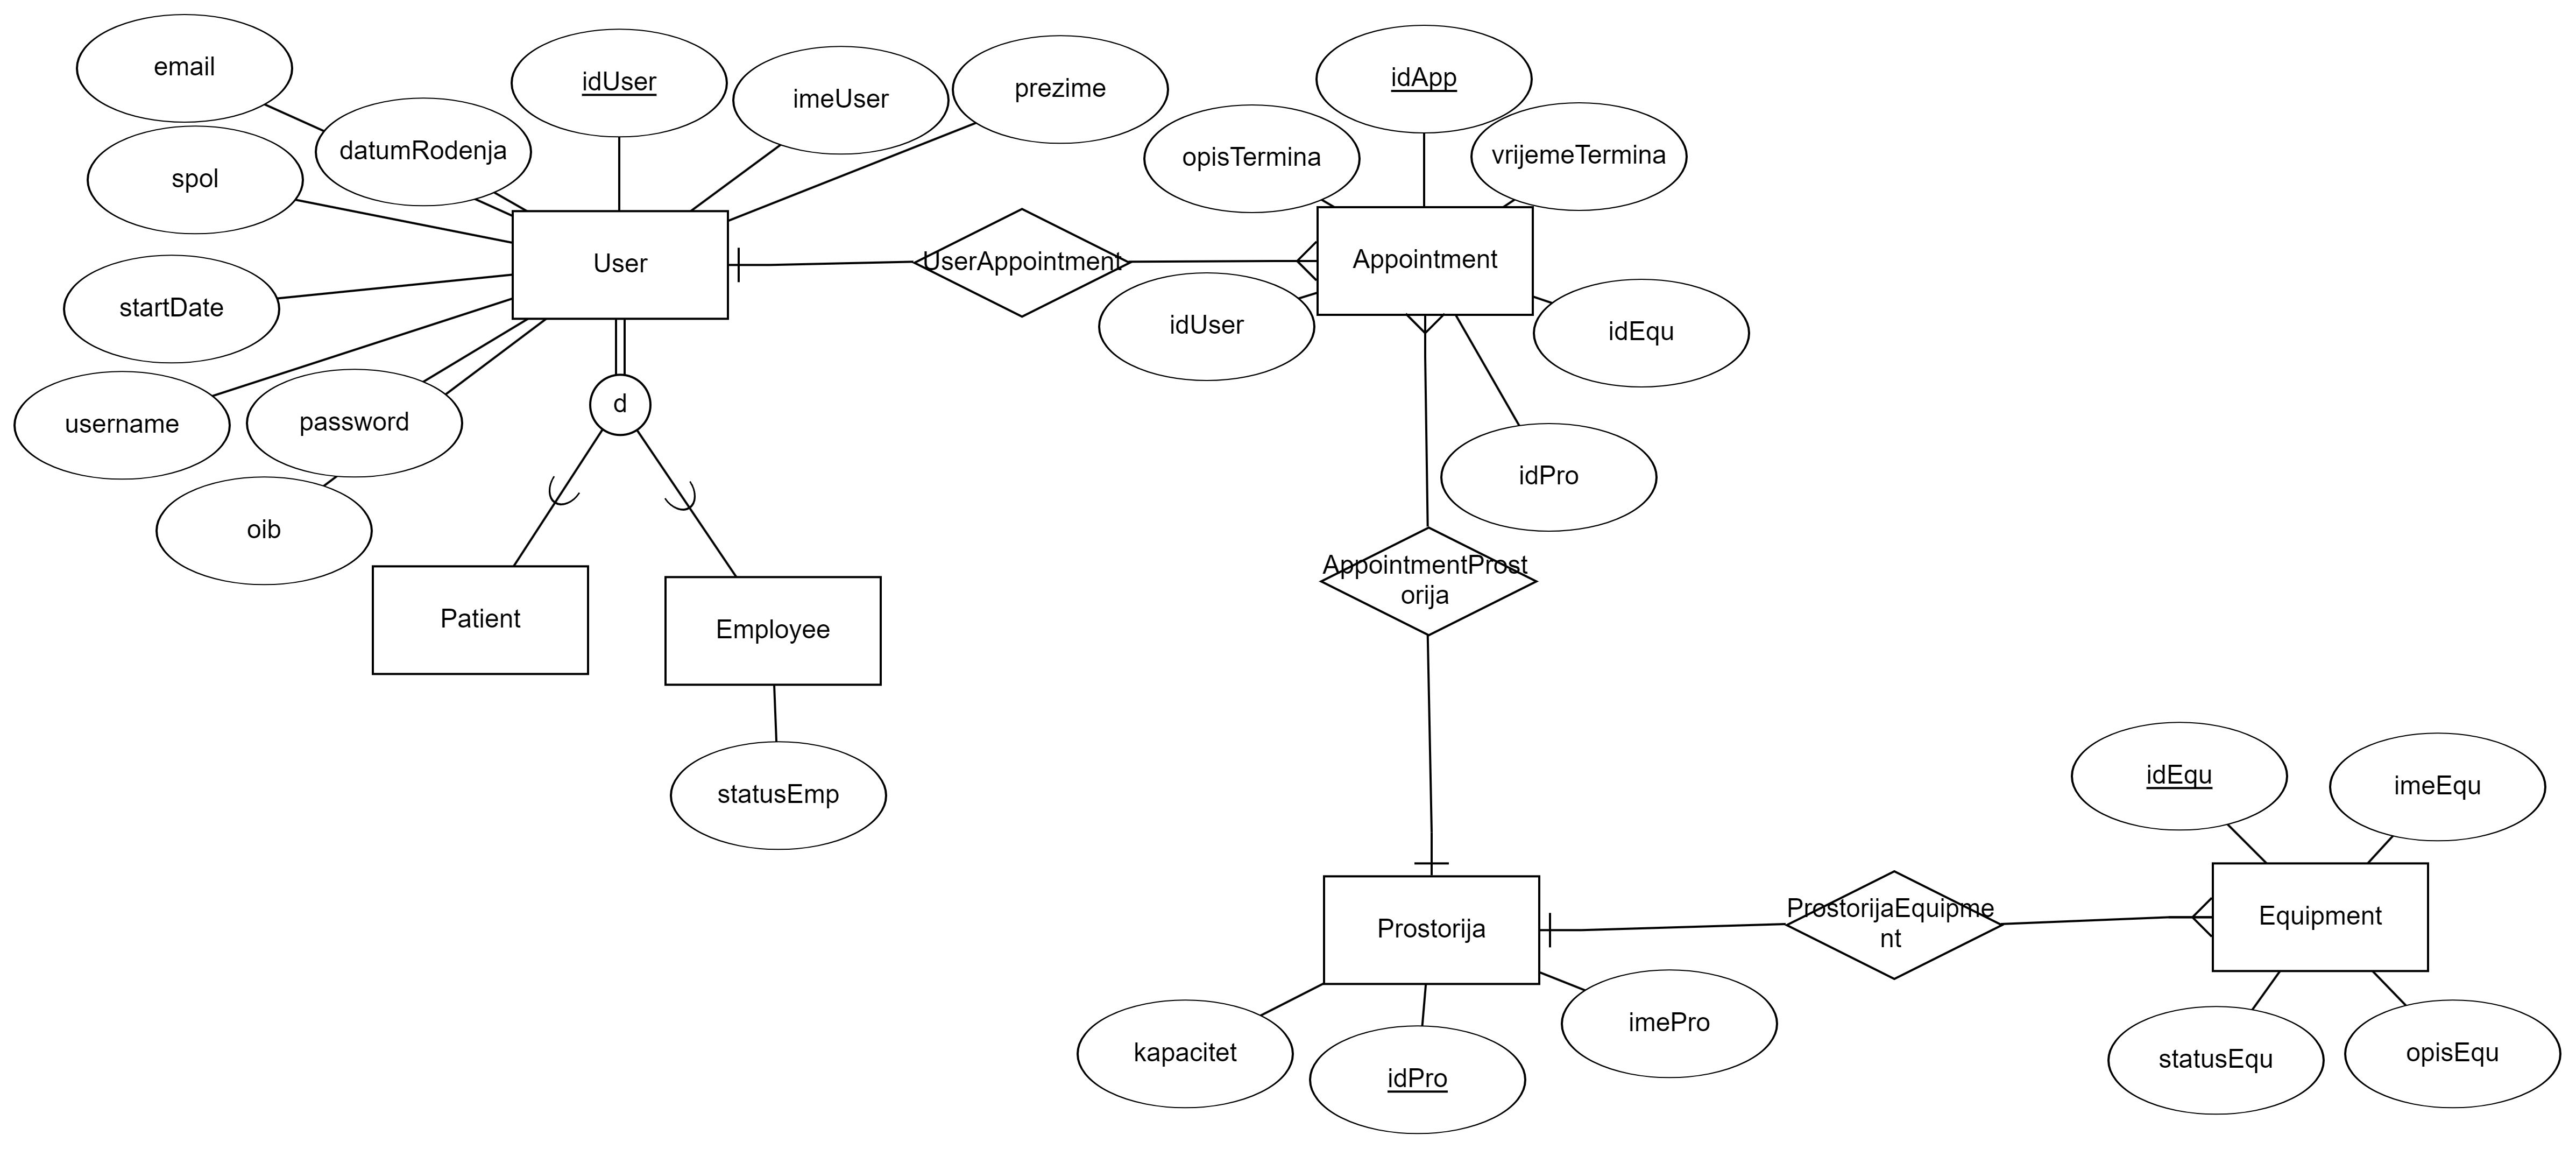
\includegraphics[scale=0.085]{slike/bp_er.PNG} %veličina slike u odnosu na originalnu datoteku i pozicija slike
					\centering
					\caption{ER model baze podataka}
					\label{fig:promjene}
				\end{figure}
			
			\eject
			
			
		\section{Dijagram razreda}
		
			\textit{Potrebno je priložiti dijagram razreda s pripadajućim opisom. Zbog preglednosti je moguće dijagram razlomiti na više njih, ali moraju biti grupirani prema sličnim razinama apstrakcije i srodnim funkcionalnostima.}\\
			
			\textbf{\textit{dio 1. revizije}}\\
			
			\textit{Prilikom prve predaje projekta, potrebno je priložiti potpuno razrađen dijagram razreda vezan uz \textbf{generičku funkcionalnost} sustava. Ostale funkcionalnosti trebaju biti idejno razrađene u dijagramu sa sljedećim komponentama: nazivi razreda, nazivi metoda i vrste pristupa metodama (npr. javni, zaštićeni), nazivi atributa razreda, veze i odnosi između razreda.}\\
			
			\textbf{\textit{dio 2. revizije}}\\			
			
			\textit{Prilikom druge predaje projekta dijagram razreda i opisi moraju odgovarati stvarnom stanju implementacije}
			
			
			
			\eject
		
		\section{Dijagram stanja}
			
			
			\textbf{\textit{dio 2. revizije}}\\
			
			\textit{Potrebno je priložiti dijagram stanja i opisati ga. Dovoljan je jedan dijagram stanja koji prikazuje \textbf{značajan dio funkcionalnosti} sustava. Na primjer, stanja korisničkog sučelja i tijek korištenja neke ključne funkcionalnosti jesu značajan dio sustava, a registracija i prijava nisu. }
			
			
			\eject 
		
		\section{Dijagram aktivnosti}
			
			\textbf{\textit{dio 2. revizije}}\\
			
			 \textit{Potrebno je priložiti dijagram aktivnosti s pripadajućim opisom. Dijagram aktivnosti treba prikazivati značajan dio sustava.}
			
			\eject
		\section{Dijagram komponenti}
		
			\textbf{\textit{dio 2. revizije}}\\
		
			 \textit{Potrebno je priložiti dijagram komponenti s pripadajućim opisom. Dijagram komponenti treba prikazivati strukturu cijele aplikacije.}
	\chapter{Implementacija i korisničko sučelje}
		
		
		\section{Korištene tehnologije i alati}
		
			
			 {Komunikacija u timu se obavljala pomoću aplikacija \underbar{WhatsApp}\footnote{Aplikacija za besplatnu razmjenu poruka, fotografija, videozapisa i drugih datoteka, te uspostavljanje glasovnih i videopoziva putem mobilnog interneta pametnim telefonima:\newline\url{https://www.whatsapp.com/}} i \underbar{Discord}\footnote{Besplatna aplikacija za komunikaciju putem tekstualnih poruka i glasovnih i video poziva:\newline\url{https://discord.com/}}.
			 	\newline Dokumentacija je bila pisana pomoću alata TeXstudio i TexLive. Za izradu UML dijagrama korišten je alat \underbar{Astah Professional}\footnote{https://astah.net/products/astah-professional/}.Kao razvojno okruženje korišten je \underbar{IntelliJ IDEA Ultimate}\footnote{https://www.jetbrains.com/lp/intellij-frameworks/}. IntelliJ IDEA je integrirano razvojno okruženje napisano u Javi za razvoj računalnog softvera napisanog u Javi, Kotlinu, Groovyju i drugim jezicima koji se temelje na JVM-u. Razvio ga je JetBrains i dostupan je u dva izdanja, Ultimate i Community. Aplikacija je napisana koristeći radni okvir \underbar{Spring Boot}\footnote{\url{https://spring.io/projects/spring-boot}} i jezik \underbar{Java}\footnote{\url{https://www.java.com/en/}} za izradu backenda. Za izradu frontenda je koristen \underbar{React}\footnote{Besplatna JavaScript biblioteka otvorenog tipa za izgradnju korisničkih sučelja:\newline\url{https://reactjs.org/}}. Za izradu naše baze podataka koristili smo \underbar{PostgreSQL}\footnote{https://www.postgresql.org/}.}
			
			
			\eject 
		
	
		\section{Ispitivanje programskog rješenja}
			
			\textbf{\textit{dio 2. revizije}}\\
			
			 \textit{U ovom poglavlju je potrebno opisati provedbu ispitivanja implementiranih funkcionalnosti na razini komponenti i na razini cijelog sustava s prikazom odabranih ispitnih slučajeva. Studenti trebaju ispitati temeljnu funkcionalnost i rubne uvjete.}
	
			
			\subsection{Ispitivanje komponenti}
			\textit{Potrebno je provesti ispitivanje jedinica (engl. unit testing) nad razredima koji implementiraju temeljne funkcionalnosti. Razraditi \textbf{minimalno 6 ispitnih slučajeva} u kojima će se ispitati redovni slučajevi, rubni uvjeti te izazivanje pogreške (engl. exception throwing). Poželjno je stvoriti i ispitni slučaj koji koristi funkcionalnosti koje nisu implementirane. Potrebno je priložiti izvorni kôd svih ispitnih slučajeva te prikaz rezultata izvođenja ispita u razvojnom okruženju (prolaz/pad ispita). }
			
			
			
			\subsection{Ispitivanje sustava}
			
			 \textit{Potrebno je provesti i opisati ispitivanje sustava koristeći radni okvir Selenium\footnote{\url{https://www.seleniumhq.org/}}. Razraditi \textbf{minimalno 4 ispitna slučaja} u kojima će se ispitati redovni slučajevi, rubni uvjeti te poziv funkcionalnosti koja nije implementirana/izaziva pogrešku kako bi se vidjelo na koji način sustav reagira kada nešto nije u potpunosti ostvareno. Ispitni slučaj se treba sastojati od ulaza (npr. korisničko ime i lozinka), očekivanog izlaza ili rezultata, koraka ispitivanja i dobivenog izlaza ili rezultata.\\ }
			 
			 \textit{Izradu ispitnih slučajeva pomoću radnog okvira Selenium moguće je provesti pomoću jednog od sljedeća dva alata:}
			 \begin{itemize}
			 	\item \textit{dodatak za preglednik \textbf{Selenium IDE} - snimanje korisnikovih akcija radi automatskog ponavljanja ispita	}
			 	\item \textit{\textbf{Selenium WebDriver} - podrška za pisanje ispita u jezicima Java, C\#, PHP koristeći posebno programsko sučelje.}
			 \end{itemize}
		 	\textit{Detalji o korištenju alata Selenium bit će prikazani na posebnom predavanju tijekom semestra.}
			
			\eject 
		
		
		\section{Dijagram razmještaja}
			
		U ovom dijagramu razmještaja opisana je programska potpora i topologija sklopov-
		lja korištena u radnom okruženju sustava. Sustav je izveden u arhitekturi ”klijent-
		poslužitelj” i podijeljen je na dva dijela, na poslužiteljsko i korisničko računalo.
		Baza podataka i web poslužitelj nalaze se na poslužiteljskom računalu, klijent se
		koristi web preglednikom kako bi pristupio web aplikaciji, a sva komunikacija
		izmedu klijenta i poslužitelja odvija se HTTPS vezom.
		
		\begin{figure}[H]
			\includegraphics[scale=0.8]{slike/Dijagram razmještaja.PNG} %veličina slike u odnosu na originalnu datoteku i pozicija slike
			\centering
			\caption{Specifikacijski dijagram razmještaja}
			\label{fig:promjene}
		\end{figure}
			
			\eject 
		
		\section{Upute za puštanje u pogon}
		
			\textbf{\textit{dio 2. revizije}}\\
		
			 \textit{U ovom poglavlju potrebno je dati upute za puštanje u pogon (engl. deployment) ostvarene aplikacije. Na primjer, za web aplikacije, opisati postupak kojim se od izvornog kôda dolazi do potpuno postavljene baze podataka i poslužitelja koji odgovara na upite korisnika. Za mobilnu aplikaciju, postupak kojim se aplikacija izgradi, te postavi na neku od trgovina. Za stolnu (engl. desktop) aplikaciju, postupak kojim se aplikacija instalira na računalo. Ukoliko mobilne i stolne aplikacije komuniciraju s poslužiteljem i/ili bazom podataka, opisati i postupak njihovog postavljanja. Pri izradi uputa preporučuje se \textbf{naglasiti korake instalacije uporabom natuknica} te koristiti što je više moguće \textbf{slike ekrana} (engl. screenshots) kako bi upute bile jasne i jednostavne za slijediti.}
			
			
			 \textit{Dovršenu aplikaciju potrebno je pokrenuti na javno dostupnom poslužitelju. Studentima se preporuča korištenje neke od sljedećih besplatnih usluga: \href{https://aws.amazon.com/}{Amazon AWS}, \href{https://azure.microsoft.com/en-us/}{Microsoft Azure} ili \href{https://www.heroku.com/}{Heroku}. Mobilne aplikacije trebaju biti objavljene na F-Droid, Google Play ili Amazon App trgovini.}
			
			
			\eject 
	\chapter{Zaključak i budući rad}

		Projektni zadatak naše grupe je bio izrada  web aplikacije koja korisnicima omogućuje jednostavno naručivanje za fizikalnu terapiju i medicinsku rehabilitaciju. Razvoj projekta je trajao 13 tjedna te smo u tom periodu ostvarili gotovo sve funkcionalnosti, a projekt smo ostvarili u dvije faze. U prvoj fazi cilj nam je bio implementirati generičke funkcionalnosti poput sustava za prijavu u stranicu, dizajniranje baze podataka i izrada početne stranice.
		Započeli smo izradu projekta upoznavanjem i raspravom o tehnologijama koje koristimo. Podijelili smo se u dvije skupine, jednu koja je radila fronted i jednu koja
		je radila backend. Relativno rano smo postavili osnovni dizaj obojih aplikacija što se pokazalo kontraproduktivno zbog manjka iskustva kod većine članova koji nisu
		bili upoznati s tim arhitekturama.
		
		U drugoj fazi bilo je potrebno dovršiti preostale funkcionalnosti, krenuli smo
		dobrim tempom, ali se je ubrzo pokazalo kako je manjak praktičnog iskustva drastično
		usporio razvoj. Sporom razvoju je doprinio i veliki broj obaveza koje su svi članovi
		imali. Iako je razvoj usporio više iskusni članovi su preuzeli inicijativu i više vremena uložili u izradu aplikacije kako bi osigurali što veću funkcionalnost.
	
	
		Radeći retrospektivu zaključujem kako možda nismo bili najfunkcionalniji i
		najorganiziraniji tim, ali smo naučili puno kako se to u budućnosti ne bi ponovilo.
		Uspješno smo riješili izazove koji su se pojavili pred nama i na samom kraju smo
		isporučili funkcionalni proizvod kojim smo izrazito zadovoljni i ponosni.
		\eject 
	\chapter*{Popis literature}
		\addcontentsline{toc}{chapter}{Popis literature}
	 	
		\begin{enumerate}
			
			
			\item  Programsko inženjerstvo, FER ZEMRIS, \url{http://www.fer.hr/predmet/proinz}
			
			\item  I. Sommerville, "Software engineering", 8th ed, Addison Wesley, 2007.
			
			\item  Nikolina Frid, Alan Jović, "Modeliranje programske potpore UML-dijagramima", listopad 2023.
			
			\item  Andrea Danzante, "Korištenje razvojnog okvira Spring Boot za
			implementaciju servisa SOAP i REST", \url{https://repozitorij.foi.unizg.hr/islandora/object/foi%3A5416/datastream/PDF/view}
			
			\item  The Unified Modeling Language, \url{https://www.uml-diagrams.org/}
			
			\item  Astah Community, \url{http://astah.net/editions/uml-new}
		\end{enumerate}
		
		 
	
	
	\begingroup
	\renewcommand*\listfigurename{Indeks slika i dijagrama}
	%\renewcommand*\listtablename{Indeks tablica}
	%\let\clearpage\relax
	\listoffigures
	%\vspace{10mm}
	%\listoftables
	\endgroup
	\addcontentsline{toc}{chapter}{Indeks slika i dijagrama}


	
	\eject 
		
	\chapter*{Dodatak: Prikaz aktivnosti grupe}
		\addcontentsline{toc}{chapter}{Dodatak: Prikaz aktivnosti grupe}
		
		\section*{Dnevnik sastajanja}
		
		\begin{packed_enum}
			\item  sastanak
			
			\item[] \begin{packed_item}
				\item Datum: 23. listopad 2023.
				\item Prisustvovali: Benjamin Gregov, Filip Grgić, Marko Lipovac, Tin Ogrizek, Bruno Petković, Filip Posavec, Neven Pralas
				\item Teme sastanka:
				\begin{packed_item}
					\item  diskusija o zadatku, organiziran cijeli plan rada
					\item  podjela tima - tko će što raditi
				\end{packed_item}
			\end{packed_item}
			
			\item  sastanak
			\item[] \begin{packed_item}
				\item Datum: u ovom formatu: 04. studenti 2023.
				\item Prisustvovali: Benjamin Gregov, Filip Grgić, Marko Lipovac, Tin Ogrizek, Bruno Petković, Filip Posavec, Neven Pralas
				\item Teme sastanka:
				\begin{packed_item}
					\item  diskusija o napretku svakog pojedinog člana tima, ali i tima zajedno
					\item  rješenje problema koji se pojavio jednom članu tima, pokušaj usmjerenja članova tima na pravi put
				\end{packed_item}
			\end{packed_item}
			
			\item  sastanak
			\item[] \begin{packed_item}
				\item Datum: u ovom formatu: 13. studenti 2023.
				\item Prisustvovali: Benjamin Gregov, Filip Grgić, Marko Lipovac, Tin Ogrizek, Bruno Petković, Filip Posavec, Neven Pralas
				\item Teme sastanka:
				\begin{packed_item}
					\item  diskusija o napretku svakog pojedinog člana tima, ali i tima zajedno
					\item  diskusija o tome što smo dobro radili za prvo bodovanje, a što trebamo u sljedećem ciklusu popraviti
					\item  završavanje projekta za prvo bodovanje projekta
				\end{packed_item}
			\end{packed_item}
			
			%
			
		\end{packed_enum}
		
		\eject
		\section*{Tablica aktivnosti}
		
			\textbf{\textit{Kontinuirano osvježavanje}}\\
			
			 \textit{Napomena: Doprinose u aktivnostima treba navesti u satima po članovima grupe po aktivnosti.}

			\begin{longtblr}[
					label=none,
				]{
					vlines,hlines,
					width = \textwidth,
					colspec={X[7, l]X[1, c]X[1, c]X[1, c]X[1, c]X[1, c]X[1, c]X[1, c]}, 
					vline{1} = {1}{text=\clap{}},
					hline{1} = {1}{text=\clap{}},
					rowhead = 1,
				} 
			
				\SetCell[c=1]{c}{} & \SetCell[c=1]{c}{\rotatebox{90}{\textbf{Ime Prezime voditelja}}} & \SetCell[c=1]{c}{\rotatebox{90}{\textbf{Ime Prezime }}} &	\SetCell[c=1]{c}{\rotatebox{90}{\textbf{Ime Prezime }}} & \SetCell[c=1]{c}{\rotatebox{90}{\textbf{Ime Prezime }}} &	\SetCell[c=1]{c}{\rotatebox{90}{\textbf{Filip Posavec }}} & \SetCell[c=1]{c}{\rotatebox{90}{\textbf{Tin Ogrizek }}} &	\SetCell[c=1]{c}{\rotatebox{90}{\textbf{Neven Pralas }}} \\  
				Upravljanje projektom 		&  &  &  &  &  &  & \\ 
				Opis projektnog zadatka 	&  &  &  &  &  &  &  3 \\ 
				
				Funkcionalni zahtjevi       &  &  &  &  &  &  &  1  \\ 
				Opis pojedinih obrazaca 	&  &  &  &  &  &  &  4  \\ 
				Dijagram obrazaca 			&  &  &  &  &  &  &  2  \\ 
				Sekvencijski dijagrami 		&  &  &  &  &  &  4  \\ 
				Opis ostalih zahtjeva 		&  &  &  &  &  &  1  \\ 

				Arhitektura i dizajn sustava	 &  &  &  &  &  1  &  &  1   \\ 
				Baza podataka				&  &  &  &  &  &  &   \\ 
				Dijagram razreda 			&  &  &  &  &  &  &   \\ 
				Dijagram stanja				&  &  &  &  &  &  &  \\ 
				Dijagram aktivnosti 		&  &  &  &  &  &  &  \\ 
				Dijagram komponenti			&  &  &  &  &  &  &  \\ 
				Korištene tehnologije i alati 		&  &  &  &  &  &  &  \\ 
				Ispitivanje programskog rješenja 	&  &  &  &  &  &  &  \\ 
				Dijagram razmještaja			&  &  &  &  &  &  &  \\ 
				Upute za puštanje u pogon 		&  &  &  &  &  &  &  \\  
				Dnevnik sastajanja 			&  &  &  &  &  &  &  1  \\ 
				Zaključak i budući rad 		&  &  &  &  &  &  &  \\  
				Popis literature 			&  &  &  &  &  &  &  \\  
				&  &  &  &  &  &  &  \\ \hline 
				\textit{Dodatne stavke kako ste podijelili izradu aplikacije} 			&  &  &  &  &  &  &  \\ 
				\textit{npr. izrada početne stranice} 				&  &  &  &  &  &  &  \\  
				\textit{izrada baze podataka} 		 			&  &  &  &  &  &  & \\  
				\textit{spajanje s bazom podataka} 							&  &  &  &  &  &  &  \\ 
				\textit{back end} 							&  &  &  &  &  &  &  \\  
				 							&  &  &  &  &  &  &\\ 
			\end{longtblr}
					
					
		\eject
		\section*{Dijagrami pregleda promjena}
		
		\textbf{\textit{dio 2. revizije}}\\
		
		\textit{Prenijeti dijagram pregleda promjena nad datotekama projekta. Potrebno je na kraju projekta generirane grafove s gitlaba prenijeti u ovo poglavlje dokumentacije. Dijagrami za vlastiti projekt se mogu preuzeti s gitlab.com stranice, u izborniku Repository, pritiskom na stavku Contributors.}
		
	


\end{document} %naredbe i tekst nakon ove naredbe ne ulaze u izgrađen dokument 


